%%%%%%%%%%%%%%%%%%% vorlage.tex %%%%%%%%%%%%%%%%%%%%%%%%%%%%%
%
% LaTeX-Vorlage zur Erstellung von Projekt-Dokumentationen
% im Fachbereich Informatik der Hochschule Trier
%
% Basis: Vorlage svmono des Springer Verlags
%
%%%%%%%%%%%%%%%%%%%%%%%%%%%%%%%%%%%%%%%%%%%%%%%%%%%%%%%%%%%%%

\documentclass[envcountsame,envcountchap, deutsch]{i-studis}

\usepackage{footnote}
\usepackage[LGR,T1]{fontenc}
\usepackage{float}
\usepackage{python}
\usepackage{xparse}
\usepackage{enumitem}
\usepackage[outputdir=../../auxil]{minted}
\usepackage{comment}
\usepackage{ulem}
\usepackage[inkscapeformat=png]{svg}
\usepackage[titles]{tocloft}
\usepackage{titlesec}
\usepackage[pdftex,plainpages=false]{hyperref}
\usepackage{xurl}
\usepackage[toc]{glossaries}
\usepackage[titletoc,title,page, header]{appendix} % Anhang
\usepackage[backend=biber, style=alphabetic, isbn=true, doi=true]{biblatex}
\usepackage{makeidx}         	% Index
\usepackage{multicol}% Zweispaltiger Index
\usepackage[threshold=0]{csquotes}
\usepackage{soul}
\usepackage{caption}
\usepackage{makecell}

\setcounter{tocdepth}{4}
\setcounter{secnumdepth}{6}

\captionsetup{font=small}
\captionsetup{labelfont=bf}

\newcommand{\textgreek}[1]{\begingroup\fontencoding{LGR}\selectfont#1\endgroup}

\BeforeBeginEnvironment{tcolorbox}{\savenotes}
\AfterEndEnvironment{tcolorbox}{\spewnotes}

%\usepackage[bottom]{footmisc}	% Erzeugung von Fu�noten

%%-----------------------------------------------------
%\newif\ifpdf
%\ifx\pdfoutput\undefined
%\pdffalse
%\else
%\pdfoutput=1
%\pdftrue
%\fi
%%--------------------------------------------------------
%\ifpdf
\usepackage[pdftex]{graphicx}
\usepackage{epstopdf}

\usepackage{tcolorbox}
\usepackage[table]{colortbl}% http://ctan.org/pkg/xcolor
%\else
%\usepackage{graphicx}
%\usepackage[plainpages=false]{hyperref}
%\fi

%%-----------------------------------------------------
\usepackage{color}				% Farbverwaltung
%\usepackage{ngerman} 			% Neue deutsche Rechtsschreibung
\usepackage[english, ngerman]{babel}

\renewcommand\appendixpagename{Anhänge}
\renewcommand\appendixtocname{Anhänge}
%%-----------------------------------------------------
% Unterscheidung für Umlaute Windows-Mac
%%-----------------------------------------------------

%\usepackage[latin1]{inputenc} 	% Ermöglicht Umlaute-Darstellung
\usepackage[utf8]{inputenc}  	% Ermöglicht Umlaute-Darstellung unter Linux (je nach verwendetem Format)

%-----------------------------------------------------
\usepackage{listings} 			% Code-Darstellung
\lstset
{
	basicstyle=\scriptsize, 	% print whole listing small
	keywordstyle=\color{blue}\bfseries,
% underlined bold black keywords
	identifierstyle=, 			% nothing happens
	commentstyle=\color{red}, 	% white comments
	stringstyle=\ttfamily, 		% typewriter type for strings
	showstringspaces=false, 	% no special string spaces
	framexleftmargin=7mm,
	tabsize=3,
	showtabs=false,
	captionpos=b,
	frame=single,
	rulesepcolor=\color{blue},
	numbers=left,
	linewidth=146mm,
	xleftmargin=8mm
}

\NewDocumentCommand{\code}{v}{%
	\texttt{\textcolor{blue}{#1}}%
}
\NewDocumentCommand{\staticcode}{v}{%
	\ul{{\texttt{\textcolor{blue}{#1}}}}%
}



\usepackage{textcomp} 			% Celsius-Darstellung
\usepackage{amssymb,amsfonts,amstext,amsmath}	% Mathematische Symbole
\usepackage[german, ruled, vlined]{algorithm2e}
\usepackage[a4paper]{geometry} % Andere Formatierung
\usepackage{bibgerm}
\usepackage{array}
\usepackage{lstmisc}
\usepackage{mathtools}
\usepackage{mdwtab}
\usepackage{datagidx}
\hyphenation{Ele-men-tar-ob-jek-te  ab-ge-tas-tet Aus-wer-tung House-holder-Matrix Le-ast-Squa-res-Al-go-ri-th-men} 		% Weitere Silbentrennung bei Bedarf angeben
\setlength{\textheight}{1.1\textheight}
\pagestyle{myheadings} 			% Erzeugt selbstdefinierte Kopfzeile
\makeindex 						% Index-Erstellung

% uncomment to hide tables, equations and figures
%\excludecomment{confidential}
%\excludecomment{figure}
%\excludecomment{equation}
%\excludecomment{table}
%\let\endfigure\relax
%\let\endtable\relax
%\let\endequation\relax


\DeclareFieldFormat{doi}{\textsc{doi}: \texttt{#1}}
\DeclareFieldFormat{isbn}{\textsc{isbn}: \texttt{#1}}

\DeclareFieldFormat{postnote}{#1}
\DeclareFieldFormat{multipostnote}{#1}

\addbibresource{literatur.bib}


\newglossarystyle{mystyle}{%
	\setglossarystyle{treegroup}%

	\renewcommand*{\glossentry}[2]{%
		\glsentryitem{##1}\textbf{\glstarget{##1}{\glossentryname{##1}}}%
		\par
		\glossentrydesc{##1}
		\par
		\vspace{1cm}
	}%
}

\setglossarystyle{mystyle}


\makenoidxglossaries
\loadglsentries{chapters/Glossar/index.tex}

%--------------------------------------------------------------------------
\begin{document}

%------------------------- Titelblatt -------------------------------------
	\title{\begin{center}
			   Repetitorium SE

			   \textbf{}\\
			   \\

			   \\
			   \small{Modul se, SS 24} \\ \small{Trier University of Applied Sciences}\\ \small{Informatik Fernstudium (M.C.Sc.)}
	\end{center}}
	\project{}
%--------------------------------------------------------------------------
	\supervisor{Titel Vorname Name} 		% Betreuer der Arbeit
	\author{\begin{center}

	\end{center}}							% Autor der Arbeit
	\address{\begin{center}
				 \small{22.05.2024\\  Thorsten Suckow-Homberg, \url{https://thorsten.suckow-homberg.de}}
	\end{center}} 							% Im Zusammenhang mit dem Datum wird hinter dem Ort ein Komma angegeben
	\submitdate{} 				% Abgabedatum
%\begingroup
%  \renewcommand{\thepage}{title}
%  \mytitlepage
%  \newpage
%\endgroup



	\begingroup
	\renewcommand{\thepage}{Titel}
	\mytitlepage
	\newpage
	\endgroup
%--------------------------------------------------------------------------
	\frontmatter
%--------------------------------------------------------------------------
	\section*{Hinweise}
Modulbegleitende (Mit-)Schrift, die sich überwiegend auf \cite{Wed09} bezieht.
	\tableofcontents 						% Inhaltsverzeichnis
%--------------------------------------------------------------------------
	\mainmatter                        		% Hauptteil (ab hier arab. Seitenzahlen)
%--------------------------------------------------------------------------
% Die Kapitel werden in separaten .tex-Dateien abgelegt und hier eingebunden.
	\part{Teil 1 - Grundlagen der Softwaretechnik und Requirements Engineering}

\vspace{2cm}
\blockquote[{\url{https://fg-swt.gi.de}\footnote{abgerufen 04.04.2024}}]{``Unter \textbf{Softwaretechnik} (engl. \textit{Software Engineering}) versteht man allgemein die (Ingenieur-) Wissenschaft, die die kosteneffiziente Entwicklung von qualitativ hochwertiger Software behandelt.``}
\vspace{2cm}
\blockquote[{\cite[247]{BMEY07}}]{
    ``The amateur software engineer is always in search
    of magic, some sensational method or tool whose
    application promises to render software development trivial. It is the mark of the professional software engineer to know that no such panacea exists.
    Amateurs often want to follow cookbook steps; professionals know that right approaches to development usually lead to inept design products, born of a
    progression of lies and behind which developers can
    shield themselves from accepting responsibility for
    earlier misguided decisions. The amateur software
    engineer either ignores documentation all together,
    or follows a process that is documentation-driven,
    worrying more about how these paper products look
    to the customer than about the substance they contain. The professional acknowledges the importance
    of creating certain documents, but never does so at
    the expense of making sensible architectural innovations.``
}

\newpage
\section*{Lernziele Teil 1}

\begin{itemize}
    \item die Aufgaben und Ziele  des Software Engineerings kennen
    \item mit den Phasen des Entwicklungszyklus und ihren Inhalten vertraut sein
    \item einen Überblick über existierende Vorgehensmodelle besitzen und ihre Anwendbarkeit auf Problemstellungen beurteilen können
    \item in der Lage sein, Anforderungen geeignet aufzunehmen und schriftlich zu erfassen
\end{itemize}

\newpage
	\chapter{Manuelle Verfahren}


\section{Lernziele}

\begin{itemize}
    \item grundlegende Arten von qualitätssichernden Maßnahmen kennen
    \item grundlegende Arten von qualitätssichernden Maßnahmen nach verschiedenen Gesichtspunkten kategorisieren können
\end{itemize}

\newpage


\section{Einleitung}

Manuelle Verfahren sind ein effektives Mittel zur Suche nach Defekten.\\
Ihr Nachteil ist, dass ihre Durchführung sehr aufwändig ist.\\
Außerdem stellen manche Prüfarten für Menschen eher eintönige und fehleranfällige Tätigkeiten dar.\\

\noindent
Verschiedene Arten von Analysen können mit extra dafür entwickelten Werkzeugen automatisiert erfolgen, und lassen sich damit damit effizienter und zuverlässiger erledigen (vgl.~\cite[27]{Wed09c})

\noindent
Mit Hilfe der \textbf{werkzeuggestützten Analyse} kann u.a

\begin{itemize}
    \item die \textbf{Einhaltung von Programmierrichtlinien} überprüft werden
    \item nach \textbf{verdächtigen Mustern} im Code gesucht werden
    \item Defekte im Code aufspüren, die durch Fehlersituationen in Programmabläufen entstehen
\end{itemize}

\section{Überblick über die Verfahren}

Passende manuelle Verfahren gibt es für verschiedene Aufgabenstellungen und Teamgrößen: Besteht das Team nur aus wenigen Personen, reicht i.d.R. ein \textbf{Gutachter}.\\
Muss ein wichtiges Dokument geprüft werden (Anforderungsdokument als Vertragsgrundlage, zentraler, sicherheitskritischer Code), untersuchen mehrere Personen systematisch den Prüfgegenstand.\\

\noindent
Verschiedene Verfahren lassen sich nach der Anzahl der Teilnehmer und dem Umfang der Untersuchung einordnen (s. Abbildung~\ref{fig:manuelleverfahren} sowie Abschnitt~\ref{sec:andere-verfahren}).

\begin{figure}
    \centering
    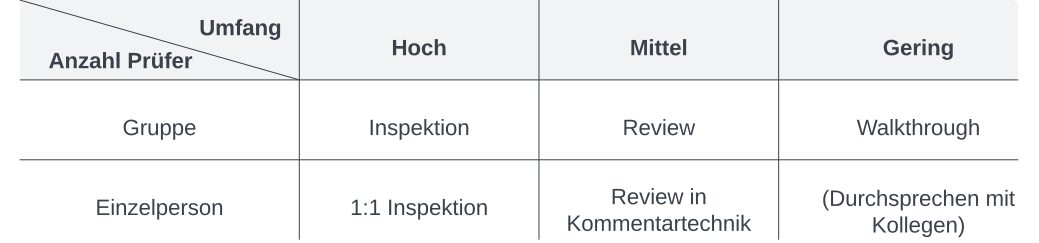
\includegraphics[scale=0.4]{part four/Manuelle Verfahren/img/manuelleverfahren}
    \caption{Verschiedene manuelle Verfahren, eingeordnet nach Anzahl der Teilnehmer und Umfang der Untersuchung. (Quelle: in Anlehnung an~\cite[Tab. 3.1, 17]{Wed09c})}
    \label{fig:manuelleverfahren}
\end{figure}

\noindent
\textbf{Inspektionen}, \textbf{Reviews} und \textbf{Walkthroughs} werden in Gruppen durchgeführt\footnote{
ergänzend führt \textit{Wedemann} als besonderes Verfahren \textbf{Pair Programming} an (vgl.~\cite[18]{Wed09c})
}.\\

\begin{itemize}
    \item \textbf{Inspektionen} sind \textbf{hoch formalisiert} und müssen von allen Beteiligten vorbereitet werden.
    \item Bei \textbf{Reviews} wird auf einen Teil der Formalisierung bei Vorbereitung und Durchführung verzichtet.\\
    \item In einem \textbf{Walkthrough} wird ein Artefakt von seinem Autor einer Gruppe von Mitarbeitern informell vorgestellt.
\end{itemize}

\section{Inspektion}
Die \textbf{Inspektion} ist das komplizierteste, aufwändigste, fromalisierteste und \textit{effektivste Verfahren}, um Defekte manuell aufzuspüren (vgl~\cite[18]{Wed09c}).\\
Alle anderen Verfahren basieren auf dem Verfahren der Inspektion.\\

\noindent
Aufgrund ihres Aufwandes kommen Inspektionen in der Praxis i.d.R. nur bei \textit{sehr wichtigen} Prüfgegenständen zum Einsatz.\\

\noindent
Bei der Inspektion wird von \textbf{Gutachtern} die \textbf{Erfüllung der Spezifikation} und die \textbf{Einhaltung von Standards} geprüft.\\
Damit nichts Wichtiges übersehen wird, werden Checklisten verwendet, die nicht unbedingt umfangreich sein müssen.\\
Die Inspektion findet zunächst alleine durch die jeweiligen Gutachter statt.
Die Ergebnisse werden in einer anschließenden \textbf{Inspektionssitzung} besprochen.

\begin{tcolorbox}[colback=white]
    Die Erarbeitung von Möglichkeiten zur Behebung von Defekten ist kein Teil der Inspektion.
\end{tcolorbox}

\subsection{Inspektionsteam}

\begin{itemize}
    \item \textbf{Moderator}: organisiert die Vorgänge der Inspektion, moderiert die Inspektionssitzung. Hat im besten Fall bereits Erfahungen mit Inspektionen gemacht und hat Kenntnisse in Gesprächsmoderation und strukturierter Arbeit mit Gruppen.
    \item \textbf{Autor(en)}: stehen während der Inspektion zur Beantwortung von Fragen zur Verfügung.
    \item \textbf{Inspektoren}: untersuchen den Prüfgegenstand, müssen also zu einer fachlichen Beurteilung in der Lage sein. Sind keine Vorgesetzten der Autoren.
    \item \textbf{Leser}: Einer der Inspektoren nimmt \textbf{während der Inspektionssitzung} die Rolle des \textbf{Lesers} ein, der durch den Prüfgegenstand führt.
\end{itemize}

\noindent
Wegen der Rollenverteilung \textbf{Leser}/\textbf{Inspektor} sollten mindestens zwei Inspektoren beteiligt sein.\\

\noindent
Das \textbf{Protokoll} führt der Moderator bei kleineren Inspektionsgruppen.\\
Bei größeren Gruppen (mehrere Inspektoren bzw. mehrere Autoren) übernimmt ein \textbf{dedizierter Protokollführer} diese Aufgabe.
\newpage


\newpage



	\chapter{Manuelle Verfahren}


\section{Lernziele}

\begin{itemize}
    \item grundlegende Arten von qualitätssichernden Maßnahmen kennen
    \item grundlegende Arten von qualitätssichernden Maßnahmen nach verschiedenen Gesichtspunkten kategorisieren können
\end{itemize}

\newpage


\section{Einleitung}

Manuelle Verfahren sind ein effektives Mittel zur Suche nach Defekten.\\
Ihr Nachteil ist, dass ihre Durchführung sehr aufwändig ist.\\
Außerdem stellen manche Prüfarten für Menschen eher eintönige und fehleranfällige Tätigkeiten dar.\\

\noindent
Verschiedene Arten von Analysen können mit extra dafür entwickelten Werkzeugen automatisiert erfolgen, und lassen sich damit damit effizienter und zuverlässiger erledigen (vgl.~\cite[27]{Wed09c})

\noindent
Mit Hilfe der \textbf{werkzeuggestützten Analyse} kann u.a

\begin{itemize}
    \item die \textbf{Einhaltung von Programmierrichtlinien} überprüft werden
    \item nach \textbf{verdächtigen Mustern} im Code gesucht werden
    \item Defekte im Code aufspüren, die durch Fehlersituationen in Programmabläufen entstehen
\end{itemize}

\section{Überblick über die Verfahren}

Passende manuelle Verfahren gibt es für verschiedene Aufgabenstellungen und Teamgrößen: Besteht das Team nur aus wenigen Personen, reicht i.d.R. ein \textbf{Gutachter}.\\
Muss ein wichtiges Dokument geprüft werden (Anforderungsdokument als Vertragsgrundlage, zentraler, sicherheitskritischer Code), untersuchen mehrere Personen systematisch den Prüfgegenstand.\\

\noindent
Verschiedene Verfahren lassen sich nach der Anzahl der Teilnehmer und dem Umfang der Untersuchung einordnen (s. Abbildung~\ref{fig:manuelleverfahren} sowie Abschnitt~\ref{sec:andere-verfahren}).

\begin{figure}
    \centering
    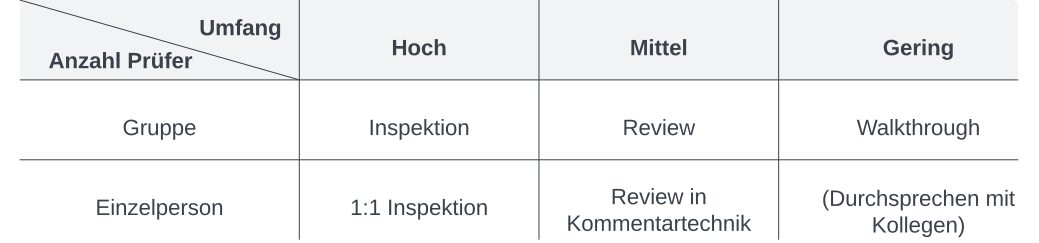
\includegraphics[scale=0.4]{part four/Manuelle Verfahren/img/manuelleverfahren}
    \caption{Verschiedene manuelle Verfahren, eingeordnet nach Anzahl der Teilnehmer und Umfang der Untersuchung. (Quelle: in Anlehnung an~\cite[Tab. 3.1, 17]{Wed09c})}
    \label{fig:manuelleverfahren}
\end{figure}

\noindent
\textbf{Inspektionen}, \textbf{Reviews} und \textbf{Walkthroughs} werden in Gruppen durchgeführt\footnote{
ergänzend führt \textit{Wedemann} als besonderes Verfahren \textbf{Pair Programming} an (vgl.~\cite[18]{Wed09c})
}.\\

\begin{itemize}
    \item \textbf{Inspektionen} sind \textbf{hoch formalisiert} und müssen von allen Beteiligten vorbereitet werden.
    \item Bei \textbf{Reviews} wird auf einen Teil der Formalisierung bei Vorbereitung und Durchführung verzichtet.\\
    \item In einem \textbf{Walkthrough} wird ein Artefakt von seinem Autor einer Gruppe von Mitarbeitern informell vorgestellt.
\end{itemize}

\section{Inspektion}
Die \textbf{Inspektion} ist das komplizierteste, aufwändigste, fromalisierteste und \textit{effektivste Verfahren}, um Defekte manuell aufzuspüren (vgl~\cite[18]{Wed09c}).\\
Alle anderen Verfahren basieren auf dem Verfahren der Inspektion.\\

\noindent
Aufgrund ihres Aufwandes kommen Inspektionen in der Praxis i.d.R. nur bei \textit{sehr wichtigen} Prüfgegenständen zum Einsatz.\\

\noindent
Bei der Inspektion wird von \textbf{Gutachtern} die \textbf{Erfüllung der Spezifikation} und die \textbf{Einhaltung von Standards} geprüft.\\
Damit nichts Wichtiges übersehen wird, werden Checklisten verwendet, die nicht unbedingt umfangreich sein müssen.\\
Die Inspektion findet zunächst alleine durch die jeweiligen Gutachter statt.
Die Ergebnisse werden in einer anschließenden \textbf{Inspektionssitzung} besprochen.

\begin{tcolorbox}[colback=white]
    Die Erarbeitung von Möglichkeiten zur Behebung von Defekten ist kein Teil der Inspektion.
\end{tcolorbox}

\subsection{Inspektionsteam}

\begin{itemize}
    \item \textbf{Moderator}: organisiert die Vorgänge der Inspektion, moderiert die Inspektionssitzung. Hat im besten Fall bereits Erfahungen mit Inspektionen gemacht und hat Kenntnisse in Gesprächsmoderation und strukturierter Arbeit mit Gruppen.
    \item \textbf{Autor(en)}: stehen während der Inspektion zur Beantwortung von Fragen zur Verfügung.
    \item \textbf{Inspektoren}: untersuchen den Prüfgegenstand, müssen also zu einer fachlichen Beurteilung in der Lage sein. Sind keine Vorgesetzten der Autoren.
    \item \textbf{Leser}: Einer der Inspektoren nimmt \textbf{während der Inspektionssitzung} die Rolle des \textbf{Lesers} ein, der durch den Prüfgegenstand führt.
\end{itemize}

\noindent
Wegen der Rollenverteilung \textbf{Leser}/\textbf{Inspektor} sollten mindestens zwei Inspektoren beteiligt sein.\\

\noindent
Das \textbf{Protokoll} führt der Moderator bei kleineren Inspektionsgruppen.\\
Bei größeren Gruppen (mehrere Inspektoren bzw. mehrere Autoren) übernimmt ein \textbf{dedizierter Protokollführer} diese Aufgabe.
\newpage


\newpage



	\chapter{Manuelle Verfahren}


\section{Lernziele}

\begin{itemize}
    \item grundlegende Arten von qualitätssichernden Maßnahmen kennen
    \item grundlegende Arten von qualitätssichernden Maßnahmen nach verschiedenen Gesichtspunkten kategorisieren können
\end{itemize}

\newpage


\section{Einleitung}

Manuelle Verfahren sind ein effektives Mittel zur Suche nach Defekten.\\
Ihr Nachteil ist, dass ihre Durchführung sehr aufwändig ist.\\
Außerdem stellen manche Prüfarten für Menschen eher eintönige und fehleranfällige Tätigkeiten dar.\\

\noindent
Verschiedene Arten von Analysen können mit extra dafür entwickelten Werkzeugen automatisiert erfolgen, und lassen sich damit damit effizienter und zuverlässiger erledigen (vgl.~\cite[27]{Wed09c})

\noindent
Mit Hilfe der \textbf{werkzeuggestützten Analyse} kann u.a

\begin{itemize}
    \item die \textbf{Einhaltung von Programmierrichtlinien} überprüft werden
    \item nach \textbf{verdächtigen Mustern} im Code gesucht werden
    \item Defekte im Code aufspüren, die durch Fehlersituationen in Programmabläufen entstehen
\end{itemize}

\section{Überblick über die Verfahren}

Passende manuelle Verfahren gibt es für verschiedene Aufgabenstellungen und Teamgrößen: Besteht das Team nur aus wenigen Personen, reicht i.d.R. ein \textbf{Gutachter}.\\
Muss ein wichtiges Dokument geprüft werden (Anforderungsdokument als Vertragsgrundlage, zentraler, sicherheitskritischer Code), untersuchen mehrere Personen systematisch den Prüfgegenstand.\\

\noindent
Verschiedene Verfahren lassen sich nach der Anzahl der Teilnehmer und dem Umfang der Untersuchung einordnen (s. Abbildung~\ref{fig:manuelleverfahren} sowie Abschnitt~\ref{sec:andere-verfahren}).

\begin{figure}
    \centering
    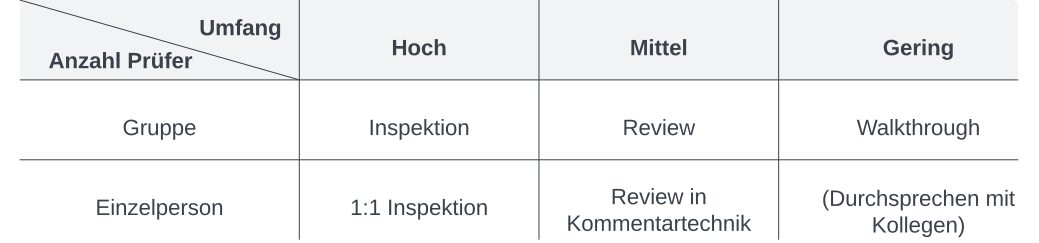
\includegraphics[scale=0.4]{part four/Manuelle Verfahren/img/manuelleverfahren}
    \caption{Verschiedene manuelle Verfahren, eingeordnet nach Anzahl der Teilnehmer und Umfang der Untersuchung. (Quelle: in Anlehnung an~\cite[Tab. 3.1, 17]{Wed09c})}
    \label{fig:manuelleverfahren}
\end{figure}

\noindent
\textbf{Inspektionen}, \textbf{Reviews} und \textbf{Walkthroughs} werden in Gruppen durchgeführt\footnote{
ergänzend führt \textit{Wedemann} als besonderes Verfahren \textbf{Pair Programming} an (vgl.~\cite[18]{Wed09c})
}.\\

\begin{itemize}
    \item \textbf{Inspektionen} sind \textbf{hoch formalisiert} und müssen von allen Beteiligten vorbereitet werden.
    \item Bei \textbf{Reviews} wird auf einen Teil der Formalisierung bei Vorbereitung und Durchführung verzichtet.\\
    \item In einem \textbf{Walkthrough} wird ein Artefakt von seinem Autor einer Gruppe von Mitarbeitern informell vorgestellt.
\end{itemize}

\section{Inspektion}
Die \textbf{Inspektion} ist das komplizierteste, aufwändigste, fromalisierteste und \textit{effektivste Verfahren}, um Defekte manuell aufzuspüren (vgl~\cite[18]{Wed09c}).\\
Alle anderen Verfahren basieren auf dem Verfahren der Inspektion.\\

\noindent
Aufgrund ihres Aufwandes kommen Inspektionen in der Praxis i.d.R. nur bei \textit{sehr wichtigen} Prüfgegenständen zum Einsatz.\\

\noindent
Bei der Inspektion wird von \textbf{Gutachtern} die \textbf{Erfüllung der Spezifikation} und die \textbf{Einhaltung von Standards} geprüft.\\
Damit nichts Wichtiges übersehen wird, werden Checklisten verwendet, die nicht unbedingt umfangreich sein müssen.\\
Die Inspektion findet zunächst alleine durch die jeweiligen Gutachter statt.
Die Ergebnisse werden in einer anschließenden \textbf{Inspektionssitzung} besprochen.

\begin{tcolorbox}[colback=white]
    Die Erarbeitung von Möglichkeiten zur Behebung von Defekten ist kein Teil der Inspektion.
\end{tcolorbox}

\subsection{Inspektionsteam}

\begin{itemize}
    \item \textbf{Moderator}: organisiert die Vorgänge der Inspektion, moderiert die Inspektionssitzung. Hat im besten Fall bereits Erfahungen mit Inspektionen gemacht und hat Kenntnisse in Gesprächsmoderation und strukturierter Arbeit mit Gruppen.
    \item \textbf{Autor(en)}: stehen während der Inspektion zur Beantwortung von Fragen zur Verfügung.
    \item \textbf{Inspektoren}: untersuchen den Prüfgegenstand, müssen also zu einer fachlichen Beurteilung in der Lage sein. Sind keine Vorgesetzten der Autoren.
    \item \textbf{Leser}: Einer der Inspektoren nimmt \textbf{während der Inspektionssitzung} die Rolle des \textbf{Lesers} ein, der durch den Prüfgegenstand führt.
\end{itemize}

\noindent
Wegen der Rollenverteilung \textbf{Leser}/\textbf{Inspektor} sollten mindestens zwei Inspektoren beteiligt sein.\\

\noindent
Das \textbf{Protokoll} führt der Moderator bei kleineren Inspektionsgruppen.\\
Bei größeren Gruppen (mehrere Inspektoren bzw. mehrere Autoren) übernimmt ein \textbf{dedizierter Protokollführer} diese Aufgabe.
\newpage


\newpage



	\chapter{Manuelle Verfahren}


\section{Lernziele}

\begin{itemize}
    \item grundlegende Arten von qualitätssichernden Maßnahmen kennen
    \item grundlegende Arten von qualitätssichernden Maßnahmen nach verschiedenen Gesichtspunkten kategorisieren können
\end{itemize}

\newpage


\section{Einleitung}

Manuelle Verfahren sind ein effektives Mittel zur Suche nach Defekten.\\
Ihr Nachteil ist, dass ihre Durchführung sehr aufwändig ist.\\
Außerdem stellen manche Prüfarten für Menschen eher eintönige und fehleranfällige Tätigkeiten dar.\\

\noindent
Verschiedene Arten von Analysen können mit extra dafür entwickelten Werkzeugen automatisiert erfolgen, und lassen sich damit damit effizienter und zuverlässiger erledigen (vgl.~\cite[27]{Wed09c})

\noindent
Mit Hilfe der \textbf{werkzeuggestützten Analyse} kann u.a

\begin{itemize}
    \item die \textbf{Einhaltung von Programmierrichtlinien} überprüft werden
    \item nach \textbf{verdächtigen Mustern} im Code gesucht werden
    \item Defekte im Code aufspüren, die durch Fehlersituationen in Programmabläufen entstehen
\end{itemize}

\section{Überblick über die Verfahren}

Passende manuelle Verfahren gibt es für verschiedene Aufgabenstellungen und Teamgrößen: Besteht das Team nur aus wenigen Personen, reicht i.d.R. ein \textbf{Gutachter}.\\
Muss ein wichtiges Dokument geprüft werden (Anforderungsdokument als Vertragsgrundlage, zentraler, sicherheitskritischer Code), untersuchen mehrere Personen systematisch den Prüfgegenstand.\\

\noindent
Verschiedene Verfahren lassen sich nach der Anzahl der Teilnehmer und dem Umfang der Untersuchung einordnen (s. Abbildung~\ref{fig:manuelleverfahren} sowie Abschnitt~\ref{sec:andere-verfahren}).

\begin{figure}
    \centering
    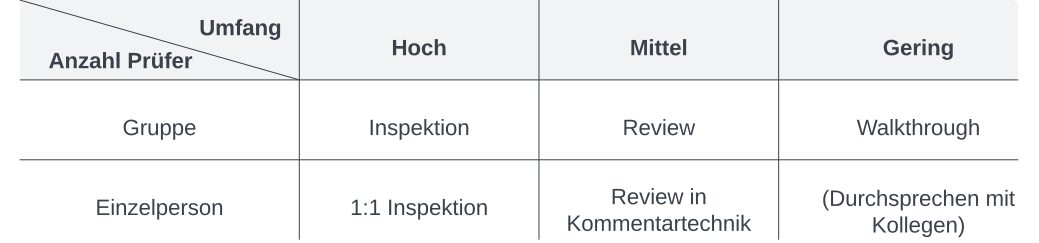
\includegraphics[scale=0.4]{part four/Manuelle Verfahren/img/manuelleverfahren}
    \caption{Verschiedene manuelle Verfahren, eingeordnet nach Anzahl der Teilnehmer und Umfang der Untersuchung. (Quelle: in Anlehnung an~\cite[Tab. 3.1, 17]{Wed09c})}
    \label{fig:manuelleverfahren}
\end{figure}

\noindent
\textbf{Inspektionen}, \textbf{Reviews} und \textbf{Walkthroughs} werden in Gruppen durchgeführt\footnote{
ergänzend führt \textit{Wedemann} als besonderes Verfahren \textbf{Pair Programming} an (vgl.~\cite[18]{Wed09c})
}.\\

\begin{itemize}
    \item \textbf{Inspektionen} sind \textbf{hoch formalisiert} und müssen von allen Beteiligten vorbereitet werden.
    \item Bei \textbf{Reviews} wird auf einen Teil der Formalisierung bei Vorbereitung und Durchführung verzichtet.\\
    \item In einem \textbf{Walkthrough} wird ein Artefakt von seinem Autor einer Gruppe von Mitarbeitern informell vorgestellt.
\end{itemize}

\section{Inspektion}
Die \textbf{Inspektion} ist das komplizierteste, aufwändigste, fromalisierteste und \textit{effektivste Verfahren}, um Defekte manuell aufzuspüren (vgl~\cite[18]{Wed09c}).\\
Alle anderen Verfahren basieren auf dem Verfahren der Inspektion.\\

\noindent
Aufgrund ihres Aufwandes kommen Inspektionen in der Praxis i.d.R. nur bei \textit{sehr wichtigen} Prüfgegenständen zum Einsatz.\\

\noindent
Bei der Inspektion wird von \textbf{Gutachtern} die \textbf{Erfüllung der Spezifikation} und die \textbf{Einhaltung von Standards} geprüft.\\
Damit nichts Wichtiges übersehen wird, werden Checklisten verwendet, die nicht unbedingt umfangreich sein müssen.\\
Die Inspektion findet zunächst alleine durch die jeweiligen Gutachter statt.
Die Ergebnisse werden in einer anschließenden \textbf{Inspektionssitzung} besprochen.

\begin{tcolorbox}[colback=white]
    Die Erarbeitung von Möglichkeiten zur Behebung von Defekten ist kein Teil der Inspektion.
\end{tcolorbox}

\subsection{Inspektionsteam}

\begin{itemize}
    \item \textbf{Moderator}: organisiert die Vorgänge der Inspektion, moderiert die Inspektionssitzung. Hat im besten Fall bereits Erfahungen mit Inspektionen gemacht und hat Kenntnisse in Gesprächsmoderation und strukturierter Arbeit mit Gruppen.
    \item \textbf{Autor(en)}: stehen während der Inspektion zur Beantwortung von Fragen zur Verfügung.
    \item \textbf{Inspektoren}: untersuchen den Prüfgegenstand, müssen also zu einer fachlichen Beurteilung in der Lage sein. Sind keine Vorgesetzten der Autoren.
    \item \textbf{Leser}: Einer der Inspektoren nimmt \textbf{während der Inspektionssitzung} die Rolle des \textbf{Lesers} ein, der durch den Prüfgegenstand führt.
\end{itemize}

\noindent
Wegen der Rollenverteilung \textbf{Leser}/\textbf{Inspektor} sollten mindestens zwei Inspektoren beteiligt sein.\\

\noindent
Das \textbf{Protokoll} führt der Moderator bei kleineren Inspektionsgruppen.\\
Bei größeren Gruppen (mehrere Inspektoren bzw. mehrere Autoren) übernimmt ein \textbf{dedizierter Protokollführer} diese Aufgabe.
\newpage


\newpage




	\part{Teil 2 - Objektorientierte Analyse und Entwurf}

\newpage
\section*{Lernziele Teil 2}

\begin{itemize}
    \item Anforderungen mit objektorientierten Methoden analysieren können
    \item systematisch eine ergonomische Benutzeroberfläche entwerfen können
    \item anhand der Anforderungen für einfache Systeme eine Architektur entwerfen können
    \item Software anhand der Analyse objektorientiert  entwerfen können, so dass sie den Anforderungen genügt
    \item bei diesen Tätigkeiten Muster einsetzen können
\end{itemize}

\newpage
	\chapter{Manuelle Verfahren}


\section{Lernziele}

\begin{itemize}
    \item grundlegende Arten von qualitätssichernden Maßnahmen kennen
    \item grundlegende Arten von qualitätssichernden Maßnahmen nach verschiedenen Gesichtspunkten kategorisieren können
\end{itemize}

\newpage


\section{Einleitung}

Manuelle Verfahren sind ein effektives Mittel zur Suche nach Defekten.\\
Ihr Nachteil ist, dass ihre Durchführung sehr aufwändig ist.\\
Außerdem stellen manche Prüfarten für Menschen eher eintönige und fehleranfällige Tätigkeiten dar.\\

\noindent
Verschiedene Arten von Analysen können mit extra dafür entwickelten Werkzeugen automatisiert erfolgen, und lassen sich damit damit effizienter und zuverlässiger erledigen (vgl.~\cite[27]{Wed09c})

\noindent
Mit Hilfe der \textbf{werkzeuggestützten Analyse} kann u.a

\begin{itemize}
    \item die \textbf{Einhaltung von Programmierrichtlinien} überprüft werden
    \item nach \textbf{verdächtigen Mustern} im Code gesucht werden
    \item Defekte im Code aufspüren, die durch Fehlersituationen in Programmabläufen entstehen
\end{itemize}

\section{Überblick über die Verfahren}

Passende manuelle Verfahren gibt es für verschiedene Aufgabenstellungen und Teamgrößen: Besteht das Team nur aus wenigen Personen, reicht i.d.R. ein \textbf{Gutachter}.\\
Muss ein wichtiges Dokument geprüft werden (Anforderungsdokument als Vertragsgrundlage, zentraler, sicherheitskritischer Code), untersuchen mehrere Personen systematisch den Prüfgegenstand.\\

\noindent
Verschiedene Verfahren lassen sich nach der Anzahl der Teilnehmer und dem Umfang der Untersuchung einordnen (s. Abbildung~\ref{fig:manuelleverfahren} sowie Abschnitt~\ref{sec:andere-verfahren}).

\begin{figure}
    \centering
    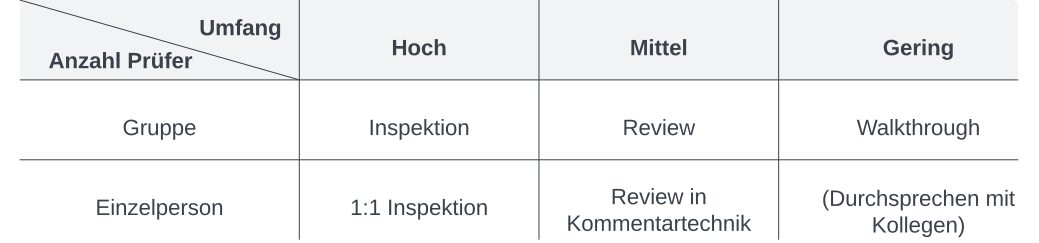
\includegraphics[scale=0.4]{part four/Manuelle Verfahren/img/manuelleverfahren}
    \caption{Verschiedene manuelle Verfahren, eingeordnet nach Anzahl der Teilnehmer und Umfang der Untersuchung. (Quelle: in Anlehnung an~\cite[Tab. 3.1, 17]{Wed09c})}
    \label{fig:manuelleverfahren}
\end{figure}

\noindent
\textbf{Inspektionen}, \textbf{Reviews} und \textbf{Walkthroughs} werden in Gruppen durchgeführt\footnote{
ergänzend führt \textit{Wedemann} als besonderes Verfahren \textbf{Pair Programming} an (vgl.~\cite[18]{Wed09c})
}.\\

\begin{itemize}
    \item \textbf{Inspektionen} sind \textbf{hoch formalisiert} und müssen von allen Beteiligten vorbereitet werden.
    \item Bei \textbf{Reviews} wird auf einen Teil der Formalisierung bei Vorbereitung und Durchführung verzichtet.\\
    \item In einem \textbf{Walkthrough} wird ein Artefakt von seinem Autor einer Gruppe von Mitarbeitern informell vorgestellt.
\end{itemize}

\section{Inspektion}
Die \textbf{Inspektion} ist das komplizierteste, aufwändigste, fromalisierteste und \textit{effektivste Verfahren}, um Defekte manuell aufzuspüren (vgl~\cite[18]{Wed09c}).\\
Alle anderen Verfahren basieren auf dem Verfahren der Inspektion.\\

\noindent
Aufgrund ihres Aufwandes kommen Inspektionen in der Praxis i.d.R. nur bei \textit{sehr wichtigen} Prüfgegenständen zum Einsatz.\\

\noindent
Bei der Inspektion wird von \textbf{Gutachtern} die \textbf{Erfüllung der Spezifikation} und die \textbf{Einhaltung von Standards} geprüft.\\
Damit nichts Wichtiges übersehen wird, werden Checklisten verwendet, die nicht unbedingt umfangreich sein müssen.\\
Die Inspektion findet zunächst alleine durch die jeweiligen Gutachter statt.
Die Ergebnisse werden in einer anschließenden \textbf{Inspektionssitzung} besprochen.

\begin{tcolorbox}[colback=white]
    Die Erarbeitung von Möglichkeiten zur Behebung von Defekten ist kein Teil der Inspektion.
\end{tcolorbox}

\subsection{Inspektionsteam}

\begin{itemize}
    \item \textbf{Moderator}: organisiert die Vorgänge der Inspektion, moderiert die Inspektionssitzung. Hat im besten Fall bereits Erfahungen mit Inspektionen gemacht und hat Kenntnisse in Gesprächsmoderation und strukturierter Arbeit mit Gruppen.
    \item \textbf{Autor(en)}: stehen während der Inspektion zur Beantwortung von Fragen zur Verfügung.
    \item \textbf{Inspektoren}: untersuchen den Prüfgegenstand, müssen also zu einer fachlichen Beurteilung in der Lage sein. Sind keine Vorgesetzten der Autoren.
    \item \textbf{Leser}: Einer der Inspektoren nimmt \textbf{während der Inspektionssitzung} die Rolle des \textbf{Lesers} ein, der durch den Prüfgegenstand führt.
\end{itemize}

\noindent
Wegen der Rollenverteilung \textbf{Leser}/\textbf{Inspektor} sollten mindestens zwei Inspektoren beteiligt sein.\\

\noindent
Das \textbf{Protokoll} führt der Moderator bei kleineren Inspektionsgruppen.\\
Bei größeren Gruppen (mehrere Inspektoren bzw. mehrere Autoren) übernimmt ein \textbf{dedizierter Protokollführer} diese Aufgabe.
\newpage


\newpage



	\chapter{Manuelle Verfahren}


\section{Lernziele}

\begin{itemize}
    \item grundlegende Arten von qualitätssichernden Maßnahmen kennen
    \item grundlegende Arten von qualitätssichernden Maßnahmen nach verschiedenen Gesichtspunkten kategorisieren können
\end{itemize}

\newpage


\section{Einleitung}

Manuelle Verfahren sind ein effektives Mittel zur Suche nach Defekten.\\
Ihr Nachteil ist, dass ihre Durchführung sehr aufwändig ist.\\
Außerdem stellen manche Prüfarten für Menschen eher eintönige und fehleranfällige Tätigkeiten dar.\\

\noindent
Verschiedene Arten von Analysen können mit extra dafür entwickelten Werkzeugen automatisiert erfolgen, und lassen sich damit damit effizienter und zuverlässiger erledigen (vgl.~\cite[27]{Wed09c})

\noindent
Mit Hilfe der \textbf{werkzeuggestützten Analyse} kann u.a

\begin{itemize}
    \item die \textbf{Einhaltung von Programmierrichtlinien} überprüft werden
    \item nach \textbf{verdächtigen Mustern} im Code gesucht werden
    \item Defekte im Code aufspüren, die durch Fehlersituationen in Programmabläufen entstehen
\end{itemize}

\section{Überblick über die Verfahren}

Passende manuelle Verfahren gibt es für verschiedene Aufgabenstellungen und Teamgrößen: Besteht das Team nur aus wenigen Personen, reicht i.d.R. ein \textbf{Gutachter}.\\
Muss ein wichtiges Dokument geprüft werden (Anforderungsdokument als Vertragsgrundlage, zentraler, sicherheitskritischer Code), untersuchen mehrere Personen systematisch den Prüfgegenstand.\\

\noindent
Verschiedene Verfahren lassen sich nach der Anzahl der Teilnehmer und dem Umfang der Untersuchung einordnen (s. Abbildung~\ref{fig:manuelleverfahren} sowie Abschnitt~\ref{sec:andere-verfahren}).

\begin{figure}
    \centering
    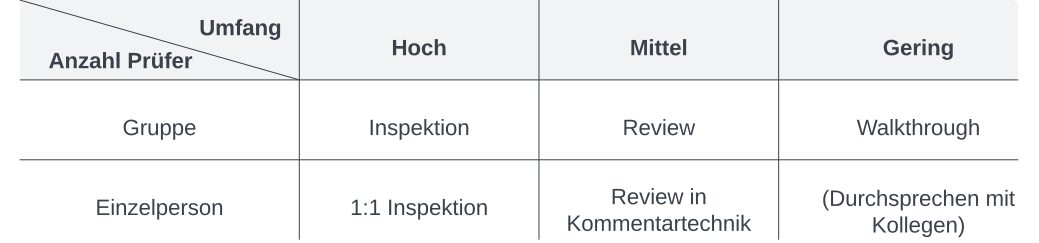
\includegraphics[scale=0.4]{part four/Manuelle Verfahren/img/manuelleverfahren}
    \caption{Verschiedene manuelle Verfahren, eingeordnet nach Anzahl der Teilnehmer und Umfang der Untersuchung. (Quelle: in Anlehnung an~\cite[Tab. 3.1, 17]{Wed09c})}
    \label{fig:manuelleverfahren}
\end{figure}

\noindent
\textbf{Inspektionen}, \textbf{Reviews} und \textbf{Walkthroughs} werden in Gruppen durchgeführt\footnote{
ergänzend führt \textit{Wedemann} als besonderes Verfahren \textbf{Pair Programming} an (vgl.~\cite[18]{Wed09c})
}.\\

\begin{itemize}
    \item \textbf{Inspektionen} sind \textbf{hoch formalisiert} und müssen von allen Beteiligten vorbereitet werden.
    \item Bei \textbf{Reviews} wird auf einen Teil der Formalisierung bei Vorbereitung und Durchführung verzichtet.\\
    \item In einem \textbf{Walkthrough} wird ein Artefakt von seinem Autor einer Gruppe von Mitarbeitern informell vorgestellt.
\end{itemize}

\section{Inspektion}
Die \textbf{Inspektion} ist das komplizierteste, aufwändigste, fromalisierteste und \textit{effektivste Verfahren}, um Defekte manuell aufzuspüren (vgl~\cite[18]{Wed09c}).\\
Alle anderen Verfahren basieren auf dem Verfahren der Inspektion.\\

\noindent
Aufgrund ihres Aufwandes kommen Inspektionen in der Praxis i.d.R. nur bei \textit{sehr wichtigen} Prüfgegenständen zum Einsatz.\\

\noindent
Bei der Inspektion wird von \textbf{Gutachtern} die \textbf{Erfüllung der Spezifikation} und die \textbf{Einhaltung von Standards} geprüft.\\
Damit nichts Wichtiges übersehen wird, werden Checklisten verwendet, die nicht unbedingt umfangreich sein müssen.\\
Die Inspektion findet zunächst alleine durch die jeweiligen Gutachter statt.
Die Ergebnisse werden in einer anschließenden \textbf{Inspektionssitzung} besprochen.

\begin{tcolorbox}[colback=white]
    Die Erarbeitung von Möglichkeiten zur Behebung von Defekten ist kein Teil der Inspektion.
\end{tcolorbox}

\subsection{Inspektionsteam}

\begin{itemize}
    \item \textbf{Moderator}: organisiert die Vorgänge der Inspektion, moderiert die Inspektionssitzung. Hat im besten Fall bereits Erfahungen mit Inspektionen gemacht und hat Kenntnisse in Gesprächsmoderation und strukturierter Arbeit mit Gruppen.
    \item \textbf{Autor(en)}: stehen während der Inspektion zur Beantwortung von Fragen zur Verfügung.
    \item \textbf{Inspektoren}: untersuchen den Prüfgegenstand, müssen also zu einer fachlichen Beurteilung in der Lage sein. Sind keine Vorgesetzten der Autoren.
    \item \textbf{Leser}: Einer der Inspektoren nimmt \textbf{während der Inspektionssitzung} die Rolle des \textbf{Lesers} ein, der durch den Prüfgegenstand führt.
\end{itemize}

\noindent
Wegen der Rollenverteilung \textbf{Leser}/\textbf{Inspektor} sollten mindestens zwei Inspektoren beteiligt sein.\\

\noindent
Das \textbf{Protokoll} führt der Moderator bei kleineren Inspektionsgruppen.\\
Bei größeren Gruppen (mehrere Inspektoren bzw. mehrere Autoren) übernimmt ein \textbf{dedizierter Protokollführer} diese Aufgabe.
\newpage


\newpage



	\chapter{Manuelle Verfahren}


\section{Lernziele}

\begin{itemize}
    \item grundlegende Arten von qualitätssichernden Maßnahmen kennen
    \item grundlegende Arten von qualitätssichernden Maßnahmen nach verschiedenen Gesichtspunkten kategorisieren können
\end{itemize}

\newpage


\section{Einleitung}

Manuelle Verfahren sind ein effektives Mittel zur Suche nach Defekten.\\
Ihr Nachteil ist, dass ihre Durchführung sehr aufwändig ist.\\
Außerdem stellen manche Prüfarten für Menschen eher eintönige und fehleranfällige Tätigkeiten dar.\\

\noindent
Verschiedene Arten von Analysen können mit extra dafür entwickelten Werkzeugen automatisiert erfolgen, und lassen sich damit damit effizienter und zuverlässiger erledigen (vgl.~\cite[27]{Wed09c})

\noindent
Mit Hilfe der \textbf{werkzeuggestützten Analyse} kann u.a

\begin{itemize}
    \item die \textbf{Einhaltung von Programmierrichtlinien} überprüft werden
    \item nach \textbf{verdächtigen Mustern} im Code gesucht werden
    \item Defekte im Code aufspüren, die durch Fehlersituationen in Programmabläufen entstehen
\end{itemize}

\section{Überblick über die Verfahren}

Passende manuelle Verfahren gibt es für verschiedene Aufgabenstellungen und Teamgrößen: Besteht das Team nur aus wenigen Personen, reicht i.d.R. ein \textbf{Gutachter}.\\
Muss ein wichtiges Dokument geprüft werden (Anforderungsdokument als Vertragsgrundlage, zentraler, sicherheitskritischer Code), untersuchen mehrere Personen systematisch den Prüfgegenstand.\\

\noindent
Verschiedene Verfahren lassen sich nach der Anzahl der Teilnehmer und dem Umfang der Untersuchung einordnen (s. Abbildung~\ref{fig:manuelleverfahren} sowie Abschnitt~\ref{sec:andere-verfahren}).

\begin{figure}
    \centering
    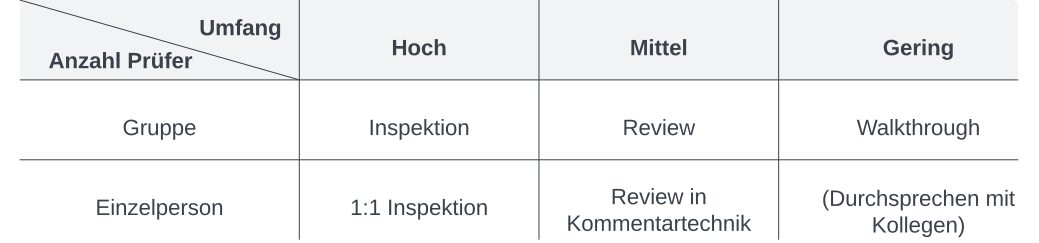
\includegraphics[scale=0.4]{part four/Manuelle Verfahren/img/manuelleverfahren}
    \caption{Verschiedene manuelle Verfahren, eingeordnet nach Anzahl der Teilnehmer und Umfang der Untersuchung. (Quelle: in Anlehnung an~\cite[Tab. 3.1, 17]{Wed09c})}
    \label{fig:manuelleverfahren}
\end{figure}

\noindent
\textbf{Inspektionen}, \textbf{Reviews} und \textbf{Walkthroughs} werden in Gruppen durchgeführt\footnote{
ergänzend führt \textit{Wedemann} als besonderes Verfahren \textbf{Pair Programming} an (vgl.~\cite[18]{Wed09c})
}.\\

\begin{itemize}
    \item \textbf{Inspektionen} sind \textbf{hoch formalisiert} und müssen von allen Beteiligten vorbereitet werden.
    \item Bei \textbf{Reviews} wird auf einen Teil der Formalisierung bei Vorbereitung und Durchführung verzichtet.\\
    \item In einem \textbf{Walkthrough} wird ein Artefakt von seinem Autor einer Gruppe von Mitarbeitern informell vorgestellt.
\end{itemize}

\section{Inspektion}
Die \textbf{Inspektion} ist das komplizierteste, aufwändigste, fromalisierteste und \textit{effektivste Verfahren}, um Defekte manuell aufzuspüren (vgl~\cite[18]{Wed09c}).\\
Alle anderen Verfahren basieren auf dem Verfahren der Inspektion.\\

\noindent
Aufgrund ihres Aufwandes kommen Inspektionen in der Praxis i.d.R. nur bei \textit{sehr wichtigen} Prüfgegenständen zum Einsatz.\\

\noindent
Bei der Inspektion wird von \textbf{Gutachtern} die \textbf{Erfüllung der Spezifikation} und die \textbf{Einhaltung von Standards} geprüft.\\
Damit nichts Wichtiges übersehen wird, werden Checklisten verwendet, die nicht unbedingt umfangreich sein müssen.\\
Die Inspektion findet zunächst alleine durch die jeweiligen Gutachter statt.
Die Ergebnisse werden in einer anschließenden \textbf{Inspektionssitzung} besprochen.

\begin{tcolorbox}[colback=white]
    Die Erarbeitung von Möglichkeiten zur Behebung von Defekten ist kein Teil der Inspektion.
\end{tcolorbox}

\subsection{Inspektionsteam}

\begin{itemize}
    \item \textbf{Moderator}: organisiert die Vorgänge der Inspektion, moderiert die Inspektionssitzung. Hat im besten Fall bereits Erfahungen mit Inspektionen gemacht und hat Kenntnisse in Gesprächsmoderation und strukturierter Arbeit mit Gruppen.
    \item \textbf{Autor(en)}: stehen während der Inspektion zur Beantwortung von Fragen zur Verfügung.
    \item \textbf{Inspektoren}: untersuchen den Prüfgegenstand, müssen also zu einer fachlichen Beurteilung in der Lage sein. Sind keine Vorgesetzten der Autoren.
    \item \textbf{Leser}: Einer der Inspektoren nimmt \textbf{während der Inspektionssitzung} die Rolle des \textbf{Lesers} ein, der durch den Prüfgegenstand führt.
\end{itemize}

\noindent
Wegen der Rollenverteilung \textbf{Leser}/\textbf{Inspektor} sollten mindestens zwei Inspektoren beteiligt sein.\\

\noindent
Das \textbf{Protokoll} führt der Moderator bei kleineren Inspektionsgruppen.\\
Bei größeren Gruppen (mehrere Inspektoren bzw. mehrere Autoren) übernimmt ein \textbf{dedizierter Protokollführer} diese Aufgabe.
\newpage


\newpage




	\part{Teil 3 - Systemmodellierung}

\newpage
\section*{Lernziele Teil 3}

\begin{itemize}
    \item den Sprachaufbau der UML 2.0 und die wesentlichen und wichtigsten Modellierungskonzepte und Diagramme beherrschen
    \item die Fähigkeit besitzen, UML 2.0 Modelle zu entwickeln
    \item in der Lage sein, UML 2.0 Modelle in der Programmiersprache Java auszudrücken
\end{itemize}

\newpage
	\chapter{Manuelle Verfahren}


\section{Lernziele}

\begin{itemize}
    \item grundlegende Arten von qualitätssichernden Maßnahmen kennen
    \item grundlegende Arten von qualitätssichernden Maßnahmen nach verschiedenen Gesichtspunkten kategorisieren können
\end{itemize}

\newpage


\section{Einleitung}

Manuelle Verfahren sind ein effektives Mittel zur Suche nach Defekten.\\
Ihr Nachteil ist, dass ihre Durchführung sehr aufwändig ist.\\
Außerdem stellen manche Prüfarten für Menschen eher eintönige und fehleranfällige Tätigkeiten dar.\\

\noindent
Verschiedene Arten von Analysen können mit extra dafür entwickelten Werkzeugen automatisiert erfolgen, und lassen sich damit damit effizienter und zuverlässiger erledigen (vgl.~\cite[27]{Wed09c})

\noindent
Mit Hilfe der \textbf{werkzeuggestützten Analyse} kann u.a

\begin{itemize}
    \item die \textbf{Einhaltung von Programmierrichtlinien} überprüft werden
    \item nach \textbf{verdächtigen Mustern} im Code gesucht werden
    \item Defekte im Code aufspüren, die durch Fehlersituationen in Programmabläufen entstehen
\end{itemize}

\section{Überblick über die Verfahren}

Passende manuelle Verfahren gibt es für verschiedene Aufgabenstellungen und Teamgrößen: Besteht das Team nur aus wenigen Personen, reicht i.d.R. ein \textbf{Gutachter}.\\
Muss ein wichtiges Dokument geprüft werden (Anforderungsdokument als Vertragsgrundlage, zentraler, sicherheitskritischer Code), untersuchen mehrere Personen systematisch den Prüfgegenstand.\\

\noindent
Verschiedene Verfahren lassen sich nach der Anzahl der Teilnehmer und dem Umfang der Untersuchung einordnen (s. Abbildung~\ref{fig:manuelleverfahren} sowie Abschnitt~\ref{sec:andere-verfahren}).

\begin{figure}
    \centering
    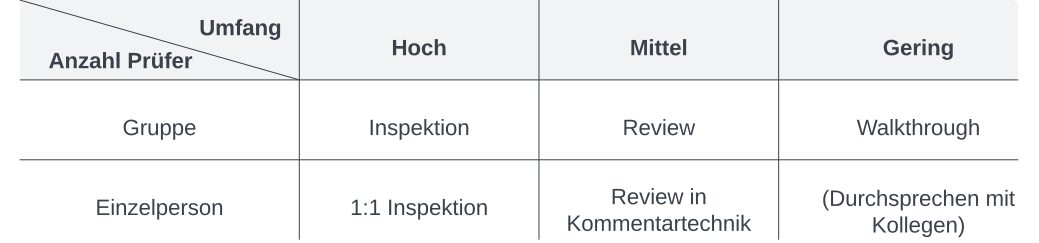
\includegraphics[scale=0.4]{part four/Manuelle Verfahren/img/manuelleverfahren}
    \caption{Verschiedene manuelle Verfahren, eingeordnet nach Anzahl der Teilnehmer und Umfang der Untersuchung. (Quelle: in Anlehnung an~\cite[Tab. 3.1, 17]{Wed09c})}
    \label{fig:manuelleverfahren}
\end{figure}

\noindent
\textbf{Inspektionen}, \textbf{Reviews} und \textbf{Walkthroughs} werden in Gruppen durchgeführt\footnote{
ergänzend führt \textit{Wedemann} als besonderes Verfahren \textbf{Pair Programming} an (vgl.~\cite[18]{Wed09c})
}.\\

\begin{itemize}
    \item \textbf{Inspektionen} sind \textbf{hoch formalisiert} und müssen von allen Beteiligten vorbereitet werden.
    \item Bei \textbf{Reviews} wird auf einen Teil der Formalisierung bei Vorbereitung und Durchführung verzichtet.\\
    \item In einem \textbf{Walkthrough} wird ein Artefakt von seinem Autor einer Gruppe von Mitarbeitern informell vorgestellt.
\end{itemize}

\section{Inspektion}
Die \textbf{Inspektion} ist das komplizierteste, aufwändigste, fromalisierteste und \textit{effektivste Verfahren}, um Defekte manuell aufzuspüren (vgl~\cite[18]{Wed09c}).\\
Alle anderen Verfahren basieren auf dem Verfahren der Inspektion.\\

\noindent
Aufgrund ihres Aufwandes kommen Inspektionen in der Praxis i.d.R. nur bei \textit{sehr wichtigen} Prüfgegenständen zum Einsatz.\\

\noindent
Bei der Inspektion wird von \textbf{Gutachtern} die \textbf{Erfüllung der Spezifikation} und die \textbf{Einhaltung von Standards} geprüft.\\
Damit nichts Wichtiges übersehen wird, werden Checklisten verwendet, die nicht unbedingt umfangreich sein müssen.\\
Die Inspektion findet zunächst alleine durch die jeweiligen Gutachter statt.
Die Ergebnisse werden in einer anschließenden \textbf{Inspektionssitzung} besprochen.

\begin{tcolorbox}[colback=white]
    Die Erarbeitung von Möglichkeiten zur Behebung von Defekten ist kein Teil der Inspektion.
\end{tcolorbox}

\subsection{Inspektionsteam}

\begin{itemize}
    \item \textbf{Moderator}: organisiert die Vorgänge der Inspektion, moderiert die Inspektionssitzung. Hat im besten Fall bereits Erfahungen mit Inspektionen gemacht und hat Kenntnisse in Gesprächsmoderation und strukturierter Arbeit mit Gruppen.
    \item \textbf{Autor(en)}: stehen während der Inspektion zur Beantwortung von Fragen zur Verfügung.
    \item \textbf{Inspektoren}: untersuchen den Prüfgegenstand, müssen also zu einer fachlichen Beurteilung in der Lage sein. Sind keine Vorgesetzten der Autoren.
    \item \textbf{Leser}: Einer der Inspektoren nimmt \textbf{während der Inspektionssitzung} die Rolle des \textbf{Lesers} ein, der durch den Prüfgegenstand führt.
\end{itemize}

\noindent
Wegen der Rollenverteilung \textbf{Leser}/\textbf{Inspektor} sollten mindestens zwei Inspektoren beteiligt sein.\\

\noindent
Das \textbf{Protokoll} führt der Moderator bei kleineren Inspektionsgruppen.\\
Bei größeren Gruppen (mehrere Inspektoren bzw. mehrere Autoren) übernimmt ein \textbf{dedizierter Protokollführer} diese Aufgabe.
\newpage


\newpage



	\chapter{Manuelle Verfahren}


\section{Lernziele}

\begin{itemize}
    \item grundlegende Arten von qualitätssichernden Maßnahmen kennen
    \item grundlegende Arten von qualitätssichernden Maßnahmen nach verschiedenen Gesichtspunkten kategorisieren können
\end{itemize}

\newpage


\section{Einleitung}

Manuelle Verfahren sind ein effektives Mittel zur Suche nach Defekten.\\
Ihr Nachteil ist, dass ihre Durchführung sehr aufwändig ist.\\
Außerdem stellen manche Prüfarten für Menschen eher eintönige und fehleranfällige Tätigkeiten dar.\\

\noindent
Verschiedene Arten von Analysen können mit extra dafür entwickelten Werkzeugen automatisiert erfolgen, und lassen sich damit damit effizienter und zuverlässiger erledigen (vgl.~\cite[27]{Wed09c})

\noindent
Mit Hilfe der \textbf{werkzeuggestützten Analyse} kann u.a

\begin{itemize}
    \item die \textbf{Einhaltung von Programmierrichtlinien} überprüft werden
    \item nach \textbf{verdächtigen Mustern} im Code gesucht werden
    \item Defekte im Code aufspüren, die durch Fehlersituationen in Programmabläufen entstehen
\end{itemize}

\section{Überblick über die Verfahren}

Passende manuelle Verfahren gibt es für verschiedene Aufgabenstellungen und Teamgrößen: Besteht das Team nur aus wenigen Personen, reicht i.d.R. ein \textbf{Gutachter}.\\
Muss ein wichtiges Dokument geprüft werden (Anforderungsdokument als Vertragsgrundlage, zentraler, sicherheitskritischer Code), untersuchen mehrere Personen systematisch den Prüfgegenstand.\\

\noindent
Verschiedene Verfahren lassen sich nach der Anzahl der Teilnehmer und dem Umfang der Untersuchung einordnen (s. Abbildung~\ref{fig:manuelleverfahren} sowie Abschnitt~\ref{sec:andere-verfahren}).

\begin{figure}
    \centering
    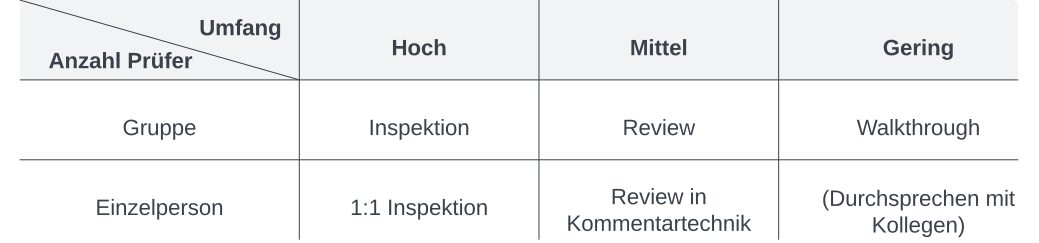
\includegraphics[scale=0.4]{part four/Manuelle Verfahren/img/manuelleverfahren}
    \caption{Verschiedene manuelle Verfahren, eingeordnet nach Anzahl der Teilnehmer und Umfang der Untersuchung. (Quelle: in Anlehnung an~\cite[Tab. 3.1, 17]{Wed09c})}
    \label{fig:manuelleverfahren}
\end{figure}

\noindent
\textbf{Inspektionen}, \textbf{Reviews} und \textbf{Walkthroughs} werden in Gruppen durchgeführt\footnote{
ergänzend führt \textit{Wedemann} als besonderes Verfahren \textbf{Pair Programming} an (vgl.~\cite[18]{Wed09c})
}.\\

\begin{itemize}
    \item \textbf{Inspektionen} sind \textbf{hoch formalisiert} und müssen von allen Beteiligten vorbereitet werden.
    \item Bei \textbf{Reviews} wird auf einen Teil der Formalisierung bei Vorbereitung und Durchführung verzichtet.\\
    \item In einem \textbf{Walkthrough} wird ein Artefakt von seinem Autor einer Gruppe von Mitarbeitern informell vorgestellt.
\end{itemize}

\section{Inspektion}
Die \textbf{Inspektion} ist das komplizierteste, aufwändigste, fromalisierteste und \textit{effektivste Verfahren}, um Defekte manuell aufzuspüren (vgl~\cite[18]{Wed09c}).\\
Alle anderen Verfahren basieren auf dem Verfahren der Inspektion.\\

\noindent
Aufgrund ihres Aufwandes kommen Inspektionen in der Praxis i.d.R. nur bei \textit{sehr wichtigen} Prüfgegenständen zum Einsatz.\\

\noindent
Bei der Inspektion wird von \textbf{Gutachtern} die \textbf{Erfüllung der Spezifikation} und die \textbf{Einhaltung von Standards} geprüft.\\
Damit nichts Wichtiges übersehen wird, werden Checklisten verwendet, die nicht unbedingt umfangreich sein müssen.\\
Die Inspektion findet zunächst alleine durch die jeweiligen Gutachter statt.
Die Ergebnisse werden in einer anschließenden \textbf{Inspektionssitzung} besprochen.

\begin{tcolorbox}[colback=white]
    Die Erarbeitung von Möglichkeiten zur Behebung von Defekten ist kein Teil der Inspektion.
\end{tcolorbox}

\subsection{Inspektionsteam}

\begin{itemize}
    \item \textbf{Moderator}: organisiert die Vorgänge der Inspektion, moderiert die Inspektionssitzung. Hat im besten Fall bereits Erfahungen mit Inspektionen gemacht und hat Kenntnisse in Gesprächsmoderation und strukturierter Arbeit mit Gruppen.
    \item \textbf{Autor(en)}: stehen während der Inspektion zur Beantwortung von Fragen zur Verfügung.
    \item \textbf{Inspektoren}: untersuchen den Prüfgegenstand, müssen also zu einer fachlichen Beurteilung in der Lage sein. Sind keine Vorgesetzten der Autoren.
    \item \textbf{Leser}: Einer der Inspektoren nimmt \textbf{während der Inspektionssitzung} die Rolle des \textbf{Lesers} ein, der durch den Prüfgegenstand führt.
\end{itemize}

\noindent
Wegen der Rollenverteilung \textbf{Leser}/\textbf{Inspektor} sollten mindestens zwei Inspektoren beteiligt sein.\\

\noindent
Das \textbf{Protokoll} führt der Moderator bei kleineren Inspektionsgruppen.\\
Bei größeren Gruppen (mehrere Inspektoren bzw. mehrere Autoren) übernimmt ein \textbf{dedizierter Protokollführer} diese Aufgabe.
\newpage


\newpage



	\chapter{Manuelle Verfahren}


\section{Lernziele}

\begin{itemize}
    \item grundlegende Arten von qualitätssichernden Maßnahmen kennen
    \item grundlegende Arten von qualitätssichernden Maßnahmen nach verschiedenen Gesichtspunkten kategorisieren können
\end{itemize}

\newpage


\section{Einleitung}

Manuelle Verfahren sind ein effektives Mittel zur Suche nach Defekten.\\
Ihr Nachteil ist, dass ihre Durchführung sehr aufwändig ist.\\
Außerdem stellen manche Prüfarten für Menschen eher eintönige und fehleranfällige Tätigkeiten dar.\\

\noindent
Verschiedene Arten von Analysen können mit extra dafür entwickelten Werkzeugen automatisiert erfolgen, und lassen sich damit damit effizienter und zuverlässiger erledigen (vgl.~\cite[27]{Wed09c})

\noindent
Mit Hilfe der \textbf{werkzeuggestützten Analyse} kann u.a

\begin{itemize}
    \item die \textbf{Einhaltung von Programmierrichtlinien} überprüft werden
    \item nach \textbf{verdächtigen Mustern} im Code gesucht werden
    \item Defekte im Code aufspüren, die durch Fehlersituationen in Programmabläufen entstehen
\end{itemize}

\section{Überblick über die Verfahren}

Passende manuelle Verfahren gibt es für verschiedene Aufgabenstellungen und Teamgrößen: Besteht das Team nur aus wenigen Personen, reicht i.d.R. ein \textbf{Gutachter}.\\
Muss ein wichtiges Dokument geprüft werden (Anforderungsdokument als Vertragsgrundlage, zentraler, sicherheitskritischer Code), untersuchen mehrere Personen systematisch den Prüfgegenstand.\\

\noindent
Verschiedene Verfahren lassen sich nach der Anzahl der Teilnehmer und dem Umfang der Untersuchung einordnen (s. Abbildung~\ref{fig:manuelleverfahren} sowie Abschnitt~\ref{sec:andere-verfahren}).

\begin{figure}
    \centering
    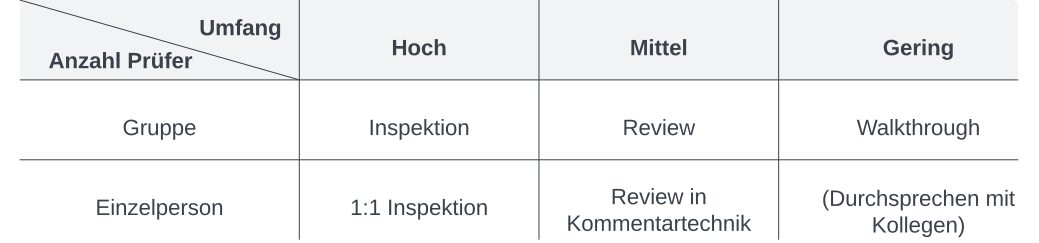
\includegraphics[scale=0.4]{part four/Manuelle Verfahren/img/manuelleverfahren}
    \caption{Verschiedene manuelle Verfahren, eingeordnet nach Anzahl der Teilnehmer und Umfang der Untersuchung. (Quelle: in Anlehnung an~\cite[Tab. 3.1, 17]{Wed09c})}
    \label{fig:manuelleverfahren}
\end{figure}

\noindent
\textbf{Inspektionen}, \textbf{Reviews} und \textbf{Walkthroughs} werden in Gruppen durchgeführt\footnote{
ergänzend führt \textit{Wedemann} als besonderes Verfahren \textbf{Pair Programming} an (vgl.~\cite[18]{Wed09c})
}.\\

\begin{itemize}
    \item \textbf{Inspektionen} sind \textbf{hoch formalisiert} und müssen von allen Beteiligten vorbereitet werden.
    \item Bei \textbf{Reviews} wird auf einen Teil der Formalisierung bei Vorbereitung und Durchführung verzichtet.\\
    \item In einem \textbf{Walkthrough} wird ein Artefakt von seinem Autor einer Gruppe von Mitarbeitern informell vorgestellt.
\end{itemize}

\section{Inspektion}
Die \textbf{Inspektion} ist das komplizierteste, aufwändigste, fromalisierteste und \textit{effektivste Verfahren}, um Defekte manuell aufzuspüren (vgl~\cite[18]{Wed09c}).\\
Alle anderen Verfahren basieren auf dem Verfahren der Inspektion.\\

\noindent
Aufgrund ihres Aufwandes kommen Inspektionen in der Praxis i.d.R. nur bei \textit{sehr wichtigen} Prüfgegenständen zum Einsatz.\\

\noindent
Bei der Inspektion wird von \textbf{Gutachtern} die \textbf{Erfüllung der Spezifikation} und die \textbf{Einhaltung von Standards} geprüft.\\
Damit nichts Wichtiges übersehen wird, werden Checklisten verwendet, die nicht unbedingt umfangreich sein müssen.\\
Die Inspektion findet zunächst alleine durch die jeweiligen Gutachter statt.
Die Ergebnisse werden in einer anschließenden \textbf{Inspektionssitzung} besprochen.

\begin{tcolorbox}[colback=white]
    Die Erarbeitung von Möglichkeiten zur Behebung von Defekten ist kein Teil der Inspektion.
\end{tcolorbox}

\subsection{Inspektionsteam}

\begin{itemize}
    \item \textbf{Moderator}: organisiert die Vorgänge der Inspektion, moderiert die Inspektionssitzung. Hat im besten Fall bereits Erfahungen mit Inspektionen gemacht und hat Kenntnisse in Gesprächsmoderation und strukturierter Arbeit mit Gruppen.
    \item \textbf{Autor(en)}: stehen während der Inspektion zur Beantwortung von Fragen zur Verfügung.
    \item \textbf{Inspektoren}: untersuchen den Prüfgegenstand, müssen also zu einer fachlichen Beurteilung in der Lage sein. Sind keine Vorgesetzten der Autoren.
    \item \textbf{Leser}: Einer der Inspektoren nimmt \textbf{während der Inspektionssitzung} die Rolle des \textbf{Lesers} ein, der durch den Prüfgegenstand führt.
\end{itemize}

\noindent
Wegen der Rollenverteilung \textbf{Leser}/\textbf{Inspektor} sollten mindestens zwei Inspektoren beteiligt sein.\\

\noindent
Das \textbf{Protokoll} führt der Moderator bei kleineren Inspektionsgruppen.\\
Bei größeren Gruppen (mehrere Inspektoren bzw. mehrere Autoren) übernimmt ein \textbf{dedizierter Protokollführer} diese Aufgabe.
\newpage


\newpage



	\chapter{Manuelle Verfahren}


\section{Lernziele}

\begin{itemize}
    \item grundlegende Arten von qualitätssichernden Maßnahmen kennen
    \item grundlegende Arten von qualitätssichernden Maßnahmen nach verschiedenen Gesichtspunkten kategorisieren können
\end{itemize}

\newpage


\section{Einleitung}

Manuelle Verfahren sind ein effektives Mittel zur Suche nach Defekten.\\
Ihr Nachteil ist, dass ihre Durchführung sehr aufwändig ist.\\
Außerdem stellen manche Prüfarten für Menschen eher eintönige und fehleranfällige Tätigkeiten dar.\\

\noindent
Verschiedene Arten von Analysen können mit extra dafür entwickelten Werkzeugen automatisiert erfolgen, und lassen sich damit damit effizienter und zuverlässiger erledigen (vgl.~\cite[27]{Wed09c})

\noindent
Mit Hilfe der \textbf{werkzeuggestützten Analyse} kann u.a

\begin{itemize}
    \item die \textbf{Einhaltung von Programmierrichtlinien} überprüft werden
    \item nach \textbf{verdächtigen Mustern} im Code gesucht werden
    \item Defekte im Code aufspüren, die durch Fehlersituationen in Programmabläufen entstehen
\end{itemize}

\section{Überblick über die Verfahren}

Passende manuelle Verfahren gibt es für verschiedene Aufgabenstellungen und Teamgrößen: Besteht das Team nur aus wenigen Personen, reicht i.d.R. ein \textbf{Gutachter}.\\
Muss ein wichtiges Dokument geprüft werden (Anforderungsdokument als Vertragsgrundlage, zentraler, sicherheitskritischer Code), untersuchen mehrere Personen systematisch den Prüfgegenstand.\\

\noindent
Verschiedene Verfahren lassen sich nach der Anzahl der Teilnehmer und dem Umfang der Untersuchung einordnen (s. Abbildung~\ref{fig:manuelleverfahren} sowie Abschnitt~\ref{sec:andere-verfahren}).

\begin{figure}
    \centering
    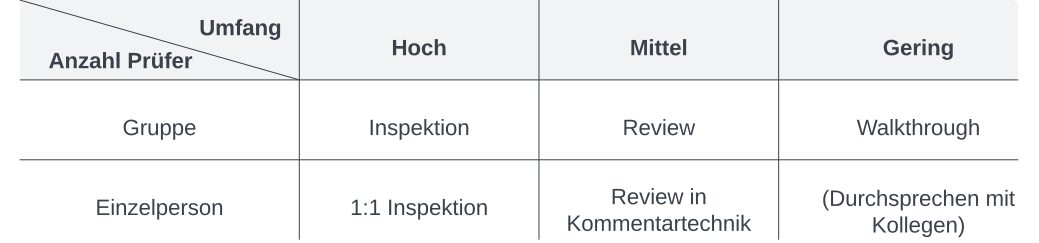
\includegraphics[scale=0.4]{part four/Manuelle Verfahren/img/manuelleverfahren}
    \caption{Verschiedene manuelle Verfahren, eingeordnet nach Anzahl der Teilnehmer und Umfang der Untersuchung. (Quelle: in Anlehnung an~\cite[Tab. 3.1, 17]{Wed09c})}
    \label{fig:manuelleverfahren}
\end{figure}

\noindent
\textbf{Inspektionen}, \textbf{Reviews} und \textbf{Walkthroughs} werden in Gruppen durchgeführt\footnote{
ergänzend führt \textit{Wedemann} als besonderes Verfahren \textbf{Pair Programming} an (vgl.~\cite[18]{Wed09c})
}.\\

\begin{itemize}
    \item \textbf{Inspektionen} sind \textbf{hoch formalisiert} und müssen von allen Beteiligten vorbereitet werden.
    \item Bei \textbf{Reviews} wird auf einen Teil der Formalisierung bei Vorbereitung und Durchführung verzichtet.\\
    \item In einem \textbf{Walkthrough} wird ein Artefakt von seinem Autor einer Gruppe von Mitarbeitern informell vorgestellt.
\end{itemize}

\section{Inspektion}
Die \textbf{Inspektion} ist das komplizierteste, aufwändigste, fromalisierteste und \textit{effektivste Verfahren}, um Defekte manuell aufzuspüren (vgl~\cite[18]{Wed09c}).\\
Alle anderen Verfahren basieren auf dem Verfahren der Inspektion.\\

\noindent
Aufgrund ihres Aufwandes kommen Inspektionen in der Praxis i.d.R. nur bei \textit{sehr wichtigen} Prüfgegenständen zum Einsatz.\\

\noindent
Bei der Inspektion wird von \textbf{Gutachtern} die \textbf{Erfüllung der Spezifikation} und die \textbf{Einhaltung von Standards} geprüft.\\
Damit nichts Wichtiges übersehen wird, werden Checklisten verwendet, die nicht unbedingt umfangreich sein müssen.\\
Die Inspektion findet zunächst alleine durch die jeweiligen Gutachter statt.
Die Ergebnisse werden in einer anschließenden \textbf{Inspektionssitzung} besprochen.

\begin{tcolorbox}[colback=white]
    Die Erarbeitung von Möglichkeiten zur Behebung von Defekten ist kein Teil der Inspektion.
\end{tcolorbox}

\subsection{Inspektionsteam}

\begin{itemize}
    \item \textbf{Moderator}: organisiert die Vorgänge der Inspektion, moderiert die Inspektionssitzung. Hat im besten Fall bereits Erfahungen mit Inspektionen gemacht und hat Kenntnisse in Gesprächsmoderation und strukturierter Arbeit mit Gruppen.
    \item \textbf{Autor(en)}: stehen während der Inspektion zur Beantwortung von Fragen zur Verfügung.
    \item \textbf{Inspektoren}: untersuchen den Prüfgegenstand, müssen also zu einer fachlichen Beurteilung in der Lage sein. Sind keine Vorgesetzten der Autoren.
    \item \textbf{Leser}: Einer der Inspektoren nimmt \textbf{während der Inspektionssitzung} die Rolle des \textbf{Lesers} ein, der durch den Prüfgegenstand führt.
\end{itemize}

\noindent
Wegen der Rollenverteilung \textbf{Leser}/\textbf{Inspektor} sollten mindestens zwei Inspektoren beteiligt sein.\\

\noindent
Das \textbf{Protokoll} führt der Moderator bei kleineren Inspektionsgruppen.\\
Bei größeren Gruppen (mehrere Inspektoren bzw. mehrere Autoren) übernimmt ein \textbf{dedizierter Protokollführer} diese Aufgabe.
\newpage


\newpage



	\chapter{Manuelle Verfahren}


\section{Lernziele}

\begin{itemize}
    \item grundlegende Arten von qualitätssichernden Maßnahmen kennen
    \item grundlegende Arten von qualitätssichernden Maßnahmen nach verschiedenen Gesichtspunkten kategorisieren können
\end{itemize}

\newpage


\section{Einleitung}

Manuelle Verfahren sind ein effektives Mittel zur Suche nach Defekten.\\
Ihr Nachteil ist, dass ihre Durchführung sehr aufwändig ist.\\
Außerdem stellen manche Prüfarten für Menschen eher eintönige und fehleranfällige Tätigkeiten dar.\\

\noindent
Verschiedene Arten von Analysen können mit extra dafür entwickelten Werkzeugen automatisiert erfolgen, und lassen sich damit damit effizienter und zuverlässiger erledigen (vgl.~\cite[27]{Wed09c})

\noindent
Mit Hilfe der \textbf{werkzeuggestützten Analyse} kann u.a

\begin{itemize}
    \item die \textbf{Einhaltung von Programmierrichtlinien} überprüft werden
    \item nach \textbf{verdächtigen Mustern} im Code gesucht werden
    \item Defekte im Code aufspüren, die durch Fehlersituationen in Programmabläufen entstehen
\end{itemize}

\section{Überblick über die Verfahren}

Passende manuelle Verfahren gibt es für verschiedene Aufgabenstellungen und Teamgrößen: Besteht das Team nur aus wenigen Personen, reicht i.d.R. ein \textbf{Gutachter}.\\
Muss ein wichtiges Dokument geprüft werden (Anforderungsdokument als Vertragsgrundlage, zentraler, sicherheitskritischer Code), untersuchen mehrere Personen systematisch den Prüfgegenstand.\\

\noindent
Verschiedene Verfahren lassen sich nach der Anzahl der Teilnehmer und dem Umfang der Untersuchung einordnen (s. Abbildung~\ref{fig:manuelleverfahren} sowie Abschnitt~\ref{sec:andere-verfahren}).

\begin{figure}
    \centering
    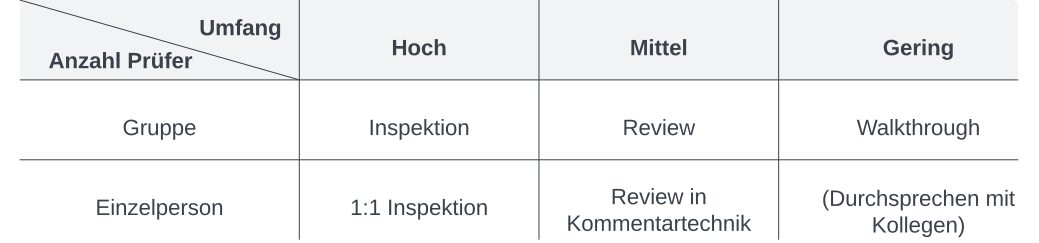
\includegraphics[scale=0.4]{part four/Manuelle Verfahren/img/manuelleverfahren}
    \caption{Verschiedene manuelle Verfahren, eingeordnet nach Anzahl der Teilnehmer und Umfang der Untersuchung. (Quelle: in Anlehnung an~\cite[Tab. 3.1, 17]{Wed09c})}
    \label{fig:manuelleverfahren}
\end{figure}

\noindent
\textbf{Inspektionen}, \textbf{Reviews} und \textbf{Walkthroughs} werden in Gruppen durchgeführt\footnote{
ergänzend führt \textit{Wedemann} als besonderes Verfahren \textbf{Pair Programming} an (vgl.~\cite[18]{Wed09c})
}.\\

\begin{itemize}
    \item \textbf{Inspektionen} sind \textbf{hoch formalisiert} und müssen von allen Beteiligten vorbereitet werden.
    \item Bei \textbf{Reviews} wird auf einen Teil der Formalisierung bei Vorbereitung und Durchführung verzichtet.\\
    \item In einem \textbf{Walkthrough} wird ein Artefakt von seinem Autor einer Gruppe von Mitarbeitern informell vorgestellt.
\end{itemize}

\section{Inspektion}
Die \textbf{Inspektion} ist das komplizierteste, aufwändigste, fromalisierteste und \textit{effektivste Verfahren}, um Defekte manuell aufzuspüren (vgl~\cite[18]{Wed09c}).\\
Alle anderen Verfahren basieren auf dem Verfahren der Inspektion.\\

\noindent
Aufgrund ihres Aufwandes kommen Inspektionen in der Praxis i.d.R. nur bei \textit{sehr wichtigen} Prüfgegenständen zum Einsatz.\\

\noindent
Bei der Inspektion wird von \textbf{Gutachtern} die \textbf{Erfüllung der Spezifikation} und die \textbf{Einhaltung von Standards} geprüft.\\
Damit nichts Wichtiges übersehen wird, werden Checklisten verwendet, die nicht unbedingt umfangreich sein müssen.\\
Die Inspektion findet zunächst alleine durch die jeweiligen Gutachter statt.
Die Ergebnisse werden in einer anschließenden \textbf{Inspektionssitzung} besprochen.

\begin{tcolorbox}[colback=white]
    Die Erarbeitung von Möglichkeiten zur Behebung von Defekten ist kein Teil der Inspektion.
\end{tcolorbox}

\subsection{Inspektionsteam}

\begin{itemize}
    \item \textbf{Moderator}: organisiert die Vorgänge der Inspektion, moderiert die Inspektionssitzung. Hat im besten Fall bereits Erfahungen mit Inspektionen gemacht und hat Kenntnisse in Gesprächsmoderation und strukturierter Arbeit mit Gruppen.
    \item \textbf{Autor(en)}: stehen während der Inspektion zur Beantwortung von Fragen zur Verfügung.
    \item \textbf{Inspektoren}: untersuchen den Prüfgegenstand, müssen also zu einer fachlichen Beurteilung in der Lage sein. Sind keine Vorgesetzten der Autoren.
    \item \textbf{Leser}: Einer der Inspektoren nimmt \textbf{während der Inspektionssitzung} die Rolle des \textbf{Lesers} ein, der durch den Prüfgegenstand führt.
\end{itemize}

\noindent
Wegen der Rollenverteilung \textbf{Leser}/\textbf{Inspektor} sollten mindestens zwei Inspektoren beteiligt sein.\\

\noindent
Das \textbf{Protokoll} führt der Moderator bei kleineren Inspektionsgruppen.\\
Bei größeren Gruppen (mehrere Inspektoren bzw. mehrere Autoren) übernimmt ein \textbf{dedizierter Protokollführer} diese Aufgabe.
\newpage


\newpage



	\chapter{Manuelle Verfahren}


\section{Lernziele}

\begin{itemize}
    \item grundlegende Arten von qualitätssichernden Maßnahmen kennen
    \item grundlegende Arten von qualitätssichernden Maßnahmen nach verschiedenen Gesichtspunkten kategorisieren können
\end{itemize}

\newpage


\section{Einleitung}

Manuelle Verfahren sind ein effektives Mittel zur Suche nach Defekten.\\
Ihr Nachteil ist, dass ihre Durchführung sehr aufwändig ist.\\
Außerdem stellen manche Prüfarten für Menschen eher eintönige und fehleranfällige Tätigkeiten dar.\\

\noindent
Verschiedene Arten von Analysen können mit extra dafür entwickelten Werkzeugen automatisiert erfolgen, und lassen sich damit damit effizienter und zuverlässiger erledigen (vgl.~\cite[27]{Wed09c})

\noindent
Mit Hilfe der \textbf{werkzeuggestützten Analyse} kann u.a

\begin{itemize}
    \item die \textbf{Einhaltung von Programmierrichtlinien} überprüft werden
    \item nach \textbf{verdächtigen Mustern} im Code gesucht werden
    \item Defekte im Code aufspüren, die durch Fehlersituationen in Programmabläufen entstehen
\end{itemize}

\section{Überblick über die Verfahren}

Passende manuelle Verfahren gibt es für verschiedene Aufgabenstellungen und Teamgrößen: Besteht das Team nur aus wenigen Personen, reicht i.d.R. ein \textbf{Gutachter}.\\
Muss ein wichtiges Dokument geprüft werden (Anforderungsdokument als Vertragsgrundlage, zentraler, sicherheitskritischer Code), untersuchen mehrere Personen systematisch den Prüfgegenstand.\\

\noindent
Verschiedene Verfahren lassen sich nach der Anzahl der Teilnehmer und dem Umfang der Untersuchung einordnen (s. Abbildung~\ref{fig:manuelleverfahren} sowie Abschnitt~\ref{sec:andere-verfahren}).

\begin{figure}
    \centering
    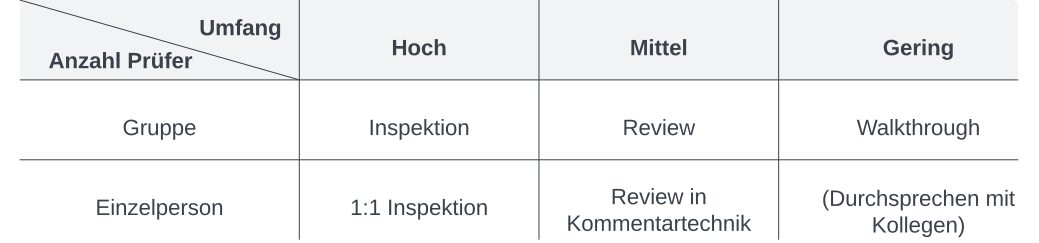
\includegraphics[scale=0.4]{part four/Manuelle Verfahren/img/manuelleverfahren}
    \caption{Verschiedene manuelle Verfahren, eingeordnet nach Anzahl der Teilnehmer und Umfang der Untersuchung. (Quelle: in Anlehnung an~\cite[Tab. 3.1, 17]{Wed09c})}
    \label{fig:manuelleverfahren}
\end{figure}

\noindent
\textbf{Inspektionen}, \textbf{Reviews} und \textbf{Walkthroughs} werden in Gruppen durchgeführt\footnote{
ergänzend führt \textit{Wedemann} als besonderes Verfahren \textbf{Pair Programming} an (vgl.~\cite[18]{Wed09c})
}.\\

\begin{itemize}
    \item \textbf{Inspektionen} sind \textbf{hoch formalisiert} und müssen von allen Beteiligten vorbereitet werden.
    \item Bei \textbf{Reviews} wird auf einen Teil der Formalisierung bei Vorbereitung und Durchführung verzichtet.\\
    \item In einem \textbf{Walkthrough} wird ein Artefakt von seinem Autor einer Gruppe von Mitarbeitern informell vorgestellt.
\end{itemize}

\section{Inspektion}
Die \textbf{Inspektion} ist das komplizierteste, aufwändigste, fromalisierteste und \textit{effektivste Verfahren}, um Defekte manuell aufzuspüren (vgl~\cite[18]{Wed09c}).\\
Alle anderen Verfahren basieren auf dem Verfahren der Inspektion.\\

\noindent
Aufgrund ihres Aufwandes kommen Inspektionen in der Praxis i.d.R. nur bei \textit{sehr wichtigen} Prüfgegenständen zum Einsatz.\\

\noindent
Bei der Inspektion wird von \textbf{Gutachtern} die \textbf{Erfüllung der Spezifikation} und die \textbf{Einhaltung von Standards} geprüft.\\
Damit nichts Wichtiges übersehen wird, werden Checklisten verwendet, die nicht unbedingt umfangreich sein müssen.\\
Die Inspektion findet zunächst alleine durch die jeweiligen Gutachter statt.
Die Ergebnisse werden in einer anschließenden \textbf{Inspektionssitzung} besprochen.

\begin{tcolorbox}[colback=white]
    Die Erarbeitung von Möglichkeiten zur Behebung von Defekten ist kein Teil der Inspektion.
\end{tcolorbox}

\subsection{Inspektionsteam}

\begin{itemize}
    \item \textbf{Moderator}: organisiert die Vorgänge der Inspektion, moderiert die Inspektionssitzung. Hat im besten Fall bereits Erfahungen mit Inspektionen gemacht und hat Kenntnisse in Gesprächsmoderation und strukturierter Arbeit mit Gruppen.
    \item \textbf{Autor(en)}: stehen während der Inspektion zur Beantwortung von Fragen zur Verfügung.
    \item \textbf{Inspektoren}: untersuchen den Prüfgegenstand, müssen also zu einer fachlichen Beurteilung in der Lage sein. Sind keine Vorgesetzten der Autoren.
    \item \textbf{Leser}: Einer der Inspektoren nimmt \textbf{während der Inspektionssitzung} die Rolle des \textbf{Lesers} ein, der durch den Prüfgegenstand führt.
\end{itemize}

\noindent
Wegen der Rollenverteilung \textbf{Leser}/\textbf{Inspektor} sollten mindestens zwei Inspektoren beteiligt sein.\\

\noindent
Das \textbf{Protokoll} führt der Moderator bei kleineren Inspektionsgruppen.\\
Bei größeren Gruppen (mehrere Inspektoren bzw. mehrere Autoren) übernimmt ein \textbf{dedizierter Protokollführer} diese Aufgabe.
\newpage


\newpage



	\chapter{Manuelle Verfahren}


\section{Lernziele}

\begin{itemize}
    \item grundlegende Arten von qualitätssichernden Maßnahmen kennen
    \item grundlegende Arten von qualitätssichernden Maßnahmen nach verschiedenen Gesichtspunkten kategorisieren können
\end{itemize}

\newpage


\section{Einleitung}

Manuelle Verfahren sind ein effektives Mittel zur Suche nach Defekten.\\
Ihr Nachteil ist, dass ihre Durchführung sehr aufwändig ist.\\
Außerdem stellen manche Prüfarten für Menschen eher eintönige und fehleranfällige Tätigkeiten dar.\\

\noindent
Verschiedene Arten von Analysen können mit extra dafür entwickelten Werkzeugen automatisiert erfolgen, und lassen sich damit damit effizienter und zuverlässiger erledigen (vgl.~\cite[27]{Wed09c})

\noindent
Mit Hilfe der \textbf{werkzeuggestützten Analyse} kann u.a

\begin{itemize}
    \item die \textbf{Einhaltung von Programmierrichtlinien} überprüft werden
    \item nach \textbf{verdächtigen Mustern} im Code gesucht werden
    \item Defekte im Code aufspüren, die durch Fehlersituationen in Programmabläufen entstehen
\end{itemize}

\section{Überblick über die Verfahren}

Passende manuelle Verfahren gibt es für verschiedene Aufgabenstellungen und Teamgrößen: Besteht das Team nur aus wenigen Personen, reicht i.d.R. ein \textbf{Gutachter}.\\
Muss ein wichtiges Dokument geprüft werden (Anforderungsdokument als Vertragsgrundlage, zentraler, sicherheitskritischer Code), untersuchen mehrere Personen systematisch den Prüfgegenstand.\\

\noindent
Verschiedene Verfahren lassen sich nach der Anzahl der Teilnehmer und dem Umfang der Untersuchung einordnen (s. Abbildung~\ref{fig:manuelleverfahren} sowie Abschnitt~\ref{sec:andere-verfahren}).

\begin{figure}
    \centering
    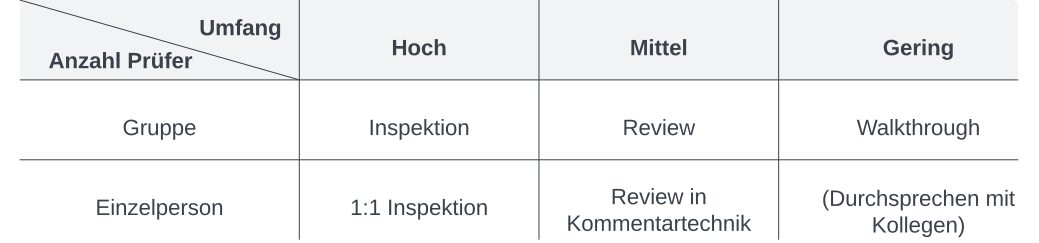
\includegraphics[scale=0.4]{part four/Manuelle Verfahren/img/manuelleverfahren}
    \caption{Verschiedene manuelle Verfahren, eingeordnet nach Anzahl der Teilnehmer und Umfang der Untersuchung. (Quelle: in Anlehnung an~\cite[Tab. 3.1, 17]{Wed09c})}
    \label{fig:manuelleverfahren}
\end{figure}

\noindent
\textbf{Inspektionen}, \textbf{Reviews} und \textbf{Walkthroughs} werden in Gruppen durchgeführt\footnote{
ergänzend führt \textit{Wedemann} als besonderes Verfahren \textbf{Pair Programming} an (vgl.~\cite[18]{Wed09c})
}.\\

\begin{itemize}
    \item \textbf{Inspektionen} sind \textbf{hoch formalisiert} und müssen von allen Beteiligten vorbereitet werden.
    \item Bei \textbf{Reviews} wird auf einen Teil der Formalisierung bei Vorbereitung und Durchführung verzichtet.\\
    \item In einem \textbf{Walkthrough} wird ein Artefakt von seinem Autor einer Gruppe von Mitarbeitern informell vorgestellt.
\end{itemize}

\section{Inspektion}
Die \textbf{Inspektion} ist das komplizierteste, aufwändigste, fromalisierteste und \textit{effektivste Verfahren}, um Defekte manuell aufzuspüren (vgl~\cite[18]{Wed09c}).\\
Alle anderen Verfahren basieren auf dem Verfahren der Inspektion.\\

\noindent
Aufgrund ihres Aufwandes kommen Inspektionen in der Praxis i.d.R. nur bei \textit{sehr wichtigen} Prüfgegenständen zum Einsatz.\\

\noindent
Bei der Inspektion wird von \textbf{Gutachtern} die \textbf{Erfüllung der Spezifikation} und die \textbf{Einhaltung von Standards} geprüft.\\
Damit nichts Wichtiges übersehen wird, werden Checklisten verwendet, die nicht unbedingt umfangreich sein müssen.\\
Die Inspektion findet zunächst alleine durch die jeweiligen Gutachter statt.
Die Ergebnisse werden in einer anschließenden \textbf{Inspektionssitzung} besprochen.

\begin{tcolorbox}[colback=white]
    Die Erarbeitung von Möglichkeiten zur Behebung von Defekten ist kein Teil der Inspektion.
\end{tcolorbox}

\subsection{Inspektionsteam}

\begin{itemize}
    \item \textbf{Moderator}: organisiert die Vorgänge der Inspektion, moderiert die Inspektionssitzung. Hat im besten Fall bereits Erfahungen mit Inspektionen gemacht und hat Kenntnisse in Gesprächsmoderation und strukturierter Arbeit mit Gruppen.
    \item \textbf{Autor(en)}: stehen während der Inspektion zur Beantwortung von Fragen zur Verfügung.
    \item \textbf{Inspektoren}: untersuchen den Prüfgegenstand, müssen also zu einer fachlichen Beurteilung in der Lage sein. Sind keine Vorgesetzten der Autoren.
    \item \textbf{Leser}: Einer der Inspektoren nimmt \textbf{während der Inspektionssitzung} die Rolle des \textbf{Lesers} ein, der durch den Prüfgegenstand führt.
\end{itemize}

\noindent
Wegen der Rollenverteilung \textbf{Leser}/\textbf{Inspektor} sollten mindestens zwei Inspektoren beteiligt sein.\\

\noindent
Das \textbf{Protokoll} führt der Moderator bei kleineren Inspektionsgruppen.\\
Bei größeren Gruppen (mehrere Inspektoren bzw. mehrere Autoren) übernimmt ein \textbf{dedizierter Protokollführer} diese Aufgabe.
\newpage


\newpage




	\part{Teil 4 - Qualitätssicherung}

\newpage
\section*{Lernziele Teil 4}

\begin{itemize}
    \item Qualität für ein Softwaresystem systematisch definieren können
    \item einen systematischen Überblick über qualitätssichernde Maßnahmen besitzen
    \item angemessene qualitätssichernde Maßnahmen für eine Aufgabe auswählen können
    \item die Qualitätssicherung in kleineren Projekten organisieren können
    \item die wichtigsten qualitätssichernden Maßnahmen wie Reviews und Tests systematisch durchführen können
    \item Werkzeuge zur Qualitätssicherung auswählen und einsetzen können
\end{itemize}

\newpage
	\chapter{Manuelle Verfahren}


\section{Lernziele}

\begin{itemize}
    \item grundlegende Arten von qualitätssichernden Maßnahmen kennen
    \item grundlegende Arten von qualitätssichernden Maßnahmen nach verschiedenen Gesichtspunkten kategorisieren können
\end{itemize}

\newpage


\section{Einleitung}

Manuelle Verfahren sind ein effektives Mittel zur Suche nach Defekten.\\
Ihr Nachteil ist, dass ihre Durchführung sehr aufwändig ist.\\
Außerdem stellen manche Prüfarten für Menschen eher eintönige und fehleranfällige Tätigkeiten dar.\\

\noindent
Verschiedene Arten von Analysen können mit extra dafür entwickelten Werkzeugen automatisiert erfolgen, und lassen sich damit damit effizienter und zuverlässiger erledigen (vgl.~\cite[27]{Wed09c})

\noindent
Mit Hilfe der \textbf{werkzeuggestützten Analyse} kann u.a

\begin{itemize}
    \item die \textbf{Einhaltung von Programmierrichtlinien} überprüft werden
    \item nach \textbf{verdächtigen Mustern} im Code gesucht werden
    \item Defekte im Code aufspüren, die durch Fehlersituationen in Programmabläufen entstehen
\end{itemize}

\section{Überblick über die Verfahren}

Passende manuelle Verfahren gibt es für verschiedene Aufgabenstellungen und Teamgrößen: Besteht das Team nur aus wenigen Personen, reicht i.d.R. ein \textbf{Gutachter}.\\
Muss ein wichtiges Dokument geprüft werden (Anforderungsdokument als Vertragsgrundlage, zentraler, sicherheitskritischer Code), untersuchen mehrere Personen systematisch den Prüfgegenstand.\\

\noindent
Verschiedene Verfahren lassen sich nach der Anzahl der Teilnehmer und dem Umfang der Untersuchung einordnen (s. Abbildung~\ref{fig:manuelleverfahren} sowie Abschnitt~\ref{sec:andere-verfahren}).

\begin{figure}
    \centering
    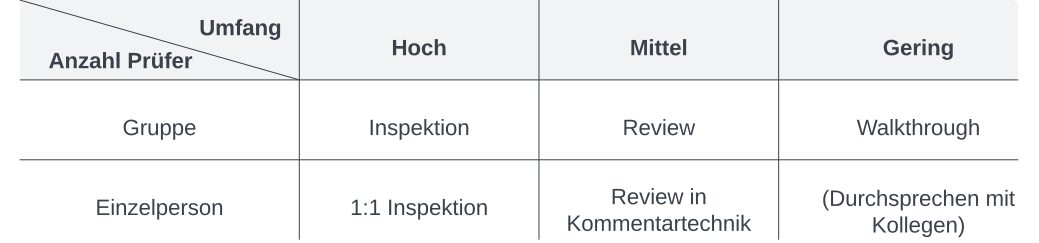
\includegraphics[scale=0.4]{part four/Manuelle Verfahren/img/manuelleverfahren}
    \caption{Verschiedene manuelle Verfahren, eingeordnet nach Anzahl der Teilnehmer und Umfang der Untersuchung. (Quelle: in Anlehnung an~\cite[Tab. 3.1, 17]{Wed09c})}
    \label{fig:manuelleverfahren}
\end{figure}

\noindent
\textbf{Inspektionen}, \textbf{Reviews} und \textbf{Walkthroughs} werden in Gruppen durchgeführt\footnote{
ergänzend führt \textit{Wedemann} als besonderes Verfahren \textbf{Pair Programming} an (vgl.~\cite[18]{Wed09c})
}.\\

\begin{itemize}
    \item \textbf{Inspektionen} sind \textbf{hoch formalisiert} und müssen von allen Beteiligten vorbereitet werden.
    \item Bei \textbf{Reviews} wird auf einen Teil der Formalisierung bei Vorbereitung und Durchführung verzichtet.\\
    \item In einem \textbf{Walkthrough} wird ein Artefakt von seinem Autor einer Gruppe von Mitarbeitern informell vorgestellt.
\end{itemize}

\section{Inspektion}
Die \textbf{Inspektion} ist das komplizierteste, aufwändigste, fromalisierteste und \textit{effektivste Verfahren}, um Defekte manuell aufzuspüren (vgl~\cite[18]{Wed09c}).\\
Alle anderen Verfahren basieren auf dem Verfahren der Inspektion.\\

\noindent
Aufgrund ihres Aufwandes kommen Inspektionen in der Praxis i.d.R. nur bei \textit{sehr wichtigen} Prüfgegenständen zum Einsatz.\\

\noindent
Bei der Inspektion wird von \textbf{Gutachtern} die \textbf{Erfüllung der Spezifikation} und die \textbf{Einhaltung von Standards} geprüft.\\
Damit nichts Wichtiges übersehen wird, werden Checklisten verwendet, die nicht unbedingt umfangreich sein müssen.\\
Die Inspektion findet zunächst alleine durch die jeweiligen Gutachter statt.
Die Ergebnisse werden in einer anschließenden \textbf{Inspektionssitzung} besprochen.

\begin{tcolorbox}[colback=white]
    Die Erarbeitung von Möglichkeiten zur Behebung von Defekten ist kein Teil der Inspektion.
\end{tcolorbox}

\subsection{Inspektionsteam}

\begin{itemize}
    \item \textbf{Moderator}: organisiert die Vorgänge der Inspektion, moderiert die Inspektionssitzung. Hat im besten Fall bereits Erfahungen mit Inspektionen gemacht und hat Kenntnisse in Gesprächsmoderation und strukturierter Arbeit mit Gruppen.
    \item \textbf{Autor(en)}: stehen während der Inspektion zur Beantwortung von Fragen zur Verfügung.
    \item \textbf{Inspektoren}: untersuchen den Prüfgegenstand, müssen also zu einer fachlichen Beurteilung in der Lage sein. Sind keine Vorgesetzten der Autoren.
    \item \textbf{Leser}: Einer der Inspektoren nimmt \textbf{während der Inspektionssitzung} die Rolle des \textbf{Lesers} ein, der durch den Prüfgegenstand führt.
\end{itemize}

\noindent
Wegen der Rollenverteilung \textbf{Leser}/\textbf{Inspektor} sollten mindestens zwei Inspektoren beteiligt sein.\\

\noindent
Das \textbf{Protokoll} führt der Moderator bei kleineren Inspektionsgruppen.\\
Bei größeren Gruppen (mehrere Inspektoren bzw. mehrere Autoren) übernimmt ein \textbf{dedizierter Protokollführer} diese Aufgabe.
\newpage


\newpage



	\chapter{Manuelle Verfahren}


\section{Lernziele}

\begin{itemize}
    \item grundlegende Arten von qualitätssichernden Maßnahmen kennen
    \item grundlegende Arten von qualitätssichernden Maßnahmen nach verschiedenen Gesichtspunkten kategorisieren können
\end{itemize}

\newpage


\section{Einleitung}

Manuelle Verfahren sind ein effektives Mittel zur Suche nach Defekten.\\
Ihr Nachteil ist, dass ihre Durchführung sehr aufwändig ist.\\
Außerdem stellen manche Prüfarten für Menschen eher eintönige und fehleranfällige Tätigkeiten dar.\\

\noindent
Verschiedene Arten von Analysen können mit extra dafür entwickelten Werkzeugen automatisiert erfolgen, und lassen sich damit damit effizienter und zuverlässiger erledigen (vgl.~\cite[27]{Wed09c})

\noindent
Mit Hilfe der \textbf{werkzeuggestützten Analyse} kann u.a

\begin{itemize}
    \item die \textbf{Einhaltung von Programmierrichtlinien} überprüft werden
    \item nach \textbf{verdächtigen Mustern} im Code gesucht werden
    \item Defekte im Code aufspüren, die durch Fehlersituationen in Programmabläufen entstehen
\end{itemize}

\section{Überblick über die Verfahren}

Passende manuelle Verfahren gibt es für verschiedene Aufgabenstellungen und Teamgrößen: Besteht das Team nur aus wenigen Personen, reicht i.d.R. ein \textbf{Gutachter}.\\
Muss ein wichtiges Dokument geprüft werden (Anforderungsdokument als Vertragsgrundlage, zentraler, sicherheitskritischer Code), untersuchen mehrere Personen systematisch den Prüfgegenstand.\\

\noindent
Verschiedene Verfahren lassen sich nach der Anzahl der Teilnehmer und dem Umfang der Untersuchung einordnen (s. Abbildung~\ref{fig:manuelleverfahren} sowie Abschnitt~\ref{sec:andere-verfahren}).

\begin{figure}
    \centering
    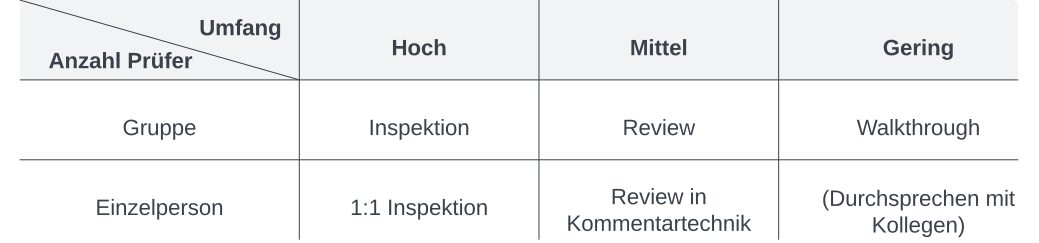
\includegraphics[scale=0.4]{part four/Manuelle Verfahren/img/manuelleverfahren}
    \caption{Verschiedene manuelle Verfahren, eingeordnet nach Anzahl der Teilnehmer und Umfang der Untersuchung. (Quelle: in Anlehnung an~\cite[Tab. 3.1, 17]{Wed09c})}
    \label{fig:manuelleverfahren}
\end{figure}

\noindent
\textbf{Inspektionen}, \textbf{Reviews} und \textbf{Walkthroughs} werden in Gruppen durchgeführt\footnote{
ergänzend führt \textit{Wedemann} als besonderes Verfahren \textbf{Pair Programming} an (vgl.~\cite[18]{Wed09c})
}.\\

\begin{itemize}
    \item \textbf{Inspektionen} sind \textbf{hoch formalisiert} und müssen von allen Beteiligten vorbereitet werden.
    \item Bei \textbf{Reviews} wird auf einen Teil der Formalisierung bei Vorbereitung und Durchführung verzichtet.\\
    \item In einem \textbf{Walkthrough} wird ein Artefakt von seinem Autor einer Gruppe von Mitarbeitern informell vorgestellt.
\end{itemize}

\section{Inspektion}
Die \textbf{Inspektion} ist das komplizierteste, aufwändigste, fromalisierteste und \textit{effektivste Verfahren}, um Defekte manuell aufzuspüren (vgl~\cite[18]{Wed09c}).\\
Alle anderen Verfahren basieren auf dem Verfahren der Inspektion.\\

\noindent
Aufgrund ihres Aufwandes kommen Inspektionen in der Praxis i.d.R. nur bei \textit{sehr wichtigen} Prüfgegenständen zum Einsatz.\\

\noindent
Bei der Inspektion wird von \textbf{Gutachtern} die \textbf{Erfüllung der Spezifikation} und die \textbf{Einhaltung von Standards} geprüft.\\
Damit nichts Wichtiges übersehen wird, werden Checklisten verwendet, die nicht unbedingt umfangreich sein müssen.\\
Die Inspektion findet zunächst alleine durch die jeweiligen Gutachter statt.
Die Ergebnisse werden in einer anschließenden \textbf{Inspektionssitzung} besprochen.

\begin{tcolorbox}[colback=white]
    Die Erarbeitung von Möglichkeiten zur Behebung von Defekten ist kein Teil der Inspektion.
\end{tcolorbox}

\subsection{Inspektionsteam}

\begin{itemize}
    \item \textbf{Moderator}: organisiert die Vorgänge der Inspektion, moderiert die Inspektionssitzung. Hat im besten Fall bereits Erfahungen mit Inspektionen gemacht und hat Kenntnisse in Gesprächsmoderation und strukturierter Arbeit mit Gruppen.
    \item \textbf{Autor(en)}: stehen während der Inspektion zur Beantwortung von Fragen zur Verfügung.
    \item \textbf{Inspektoren}: untersuchen den Prüfgegenstand, müssen also zu einer fachlichen Beurteilung in der Lage sein. Sind keine Vorgesetzten der Autoren.
    \item \textbf{Leser}: Einer der Inspektoren nimmt \textbf{während der Inspektionssitzung} die Rolle des \textbf{Lesers} ein, der durch den Prüfgegenstand führt.
\end{itemize}

\noindent
Wegen der Rollenverteilung \textbf{Leser}/\textbf{Inspektor} sollten mindestens zwei Inspektoren beteiligt sein.\\

\noindent
Das \textbf{Protokoll} führt der Moderator bei kleineren Inspektionsgruppen.\\
Bei größeren Gruppen (mehrere Inspektoren bzw. mehrere Autoren) übernimmt ein \textbf{dedizierter Protokollführer} diese Aufgabe.
\newpage


\newpage



	\chapter{Manuelle Verfahren}


\section{Lernziele}

\begin{itemize}
    \item grundlegende Arten von qualitätssichernden Maßnahmen kennen
    \item grundlegende Arten von qualitätssichernden Maßnahmen nach verschiedenen Gesichtspunkten kategorisieren können
\end{itemize}

\newpage


\section{Einleitung}

Manuelle Verfahren sind ein effektives Mittel zur Suche nach Defekten.\\
Ihr Nachteil ist, dass ihre Durchführung sehr aufwändig ist.\\
Außerdem stellen manche Prüfarten für Menschen eher eintönige und fehleranfällige Tätigkeiten dar.\\

\noindent
Verschiedene Arten von Analysen können mit extra dafür entwickelten Werkzeugen automatisiert erfolgen, und lassen sich damit damit effizienter und zuverlässiger erledigen (vgl.~\cite[27]{Wed09c})

\noindent
Mit Hilfe der \textbf{werkzeuggestützten Analyse} kann u.a

\begin{itemize}
    \item die \textbf{Einhaltung von Programmierrichtlinien} überprüft werden
    \item nach \textbf{verdächtigen Mustern} im Code gesucht werden
    \item Defekte im Code aufspüren, die durch Fehlersituationen in Programmabläufen entstehen
\end{itemize}

\section{Überblick über die Verfahren}

Passende manuelle Verfahren gibt es für verschiedene Aufgabenstellungen und Teamgrößen: Besteht das Team nur aus wenigen Personen, reicht i.d.R. ein \textbf{Gutachter}.\\
Muss ein wichtiges Dokument geprüft werden (Anforderungsdokument als Vertragsgrundlage, zentraler, sicherheitskritischer Code), untersuchen mehrere Personen systematisch den Prüfgegenstand.\\

\noindent
Verschiedene Verfahren lassen sich nach der Anzahl der Teilnehmer und dem Umfang der Untersuchung einordnen (s. Abbildung~\ref{fig:manuelleverfahren} sowie Abschnitt~\ref{sec:andere-verfahren}).

\begin{figure}
    \centering
    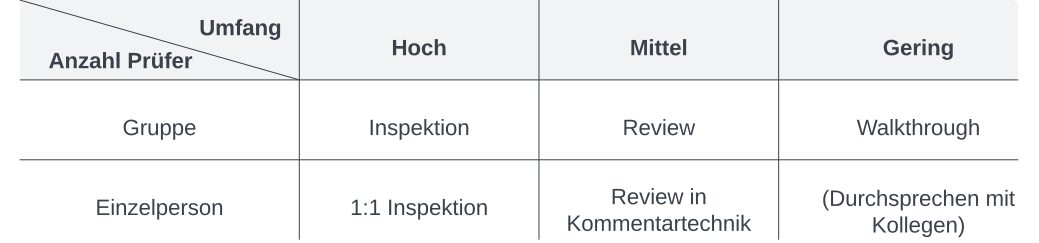
\includegraphics[scale=0.4]{part four/Manuelle Verfahren/img/manuelleverfahren}
    \caption{Verschiedene manuelle Verfahren, eingeordnet nach Anzahl der Teilnehmer und Umfang der Untersuchung. (Quelle: in Anlehnung an~\cite[Tab. 3.1, 17]{Wed09c})}
    \label{fig:manuelleverfahren}
\end{figure}

\noindent
\textbf{Inspektionen}, \textbf{Reviews} und \textbf{Walkthroughs} werden in Gruppen durchgeführt\footnote{
ergänzend führt \textit{Wedemann} als besonderes Verfahren \textbf{Pair Programming} an (vgl.~\cite[18]{Wed09c})
}.\\

\begin{itemize}
    \item \textbf{Inspektionen} sind \textbf{hoch formalisiert} und müssen von allen Beteiligten vorbereitet werden.
    \item Bei \textbf{Reviews} wird auf einen Teil der Formalisierung bei Vorbereitung und Durchführung verzichtet.\\
    \item In einem \textbf{Walkthrough} wird ein Artefakt von seinem Autor einer Gruppe von Mitarbeitern informell vorgestellt.
\end{itemize}

\section{Inspektion}
Die \textbf{Inspektion} ist das komplizierteste, aufwändigste, fromalisierteste und \textit{effektivste Verfahren}, um Defekte manuell aufzuspüren (vgl~\cite[18]{Wed09c}).\\
Alle anderen Verfahren basieren auf dem Verfahren der Inspektion.\\

\noindent
Aufgrund ihres Aufwandes kommen Inspektionen in der Praxis i.d.R. nur bei \textit{sehr wichtigen} Prüfgegenständen zum Einsatz.\\

\noindent
Bei der Inspektion wird von \textbf{Gutachtern} die \textbf{Erfüllung der Spezifikation} und die \textbf{Einhaltung von Standards} geprüft.\\
Damit nichts Wichtiges übersehen wird, werden Checklisten verwendet, die nicht unbedingt umfangreich sein müssen.\\
Die Inspektion findet zunächst alleine durch die jeweiligen Gutachter statt.
Die Ergebnisse werden in einer anschließenden \textbf{Inspektionssitzung} besprochen.

\begin{tcolorbox}[colback=white]
    Die Erarbeitung von Möglichkeiten zur Behebung von Defekten ist kein Teil der Inspektion.
\end{tcolorbox}

\subsection{Inspektionsteam}

\begin{itemize}
    \item \textbf{Moderator}: organisiert die Vorgänge der Inspektion, moderiert die Inspektionssitzung. Hat im besten Fall bereits Erfahungen mit Inspektionen gemacht und hat Kenntnisse in Gesprächsmoderation und strukturierter Arbeit mit Gruppen.
    \item \textbf{Autor(en)}: stehen während der Inspektion zur Beantwortung von Fragen zur Verfügung.
    \item \textbf{Inspektoren}: untersuchen den Prüfgegenstand, müssen also zu einer fachlichen Beurteilung in der Lage sein. Sind keine Vorgesetzten der Autoren.
    \item \textbf{Leser}: Einer der Inspektoren nimmt \textbf{während der Inspektionssitzung} die Rolle des \textbf{Lesers} ein, der durch den Prüfgegenstand führt.
\end{itemize}

\noindent
Wegen der Rollenverteilung \textbf{Leser}/\textbf{Inspektor} sollten mindestens zwei Inspektoren beteiligt sein.\\

\noindent
Das \textbf{Protokoll} führt der Moderator bei kleineren Inspektionsgruppen.\\
Bei größeren Gruppen (mehrere Inspektoren bzw. mehrere Autoren) übernimmt ein \textbf{dedizierter Protokollführer} diese Aufgabe.
\newpage


\newpage



	\chapter{Manuelle Verfahren}


\section{Lernziele}

\begin{itemize}
    \item grundlegende Arten von qualitätssichernden Maßnahmen kennen
    \item grundlegende Arten von qualitätssichernden Maßnahmen nach verschiedenen Gesichtspunkten kategorisieren können
\end{itemize}

\newpage


\section{Einleitung}

Manuelle Verfahren sind ein effektives Mittel zur Suche nach Defekten.\\
Ihr Nachteil ist, dass ihre Durchführung sehr aufwändig ist.\\
Außerdem stellen manche Prüfarten für Menschen eher eintönige und fehleranfällige Tätigkeiten dar.\\

\noindent
Verschiedene Arten von Analysen können mit extra dafür entwickelten Werkzeugen automatisiert erfolgen, und lassen sich damit damit effizienter und zuverlässiger erledigen (vgl.~\cite[27]{Wed09c})

\noindent
Mit Hilfe der \textbf{werkzeuggestützten Analyse} kann u.a

\begin{itemize}
    \item die \textbf{Einhaltung von Programmierrichtlinien} überprüft werden
    \item nach \textbf{verdächtigen Mustern} im Code gesucht werden
    \item Defekte im Code aufspüren, die durch Fehlersituationen in Programmabläufen entstehen
\end{itemize}

\section{Überblick über die Verfahren}

Passende manuelle Verfahren gibt es für verschiedene Aufgabenstellungen und Teamgrößen: Besteht das Team nur aus wenigen Personen, reicht i.d.R. ein \textbf{Gutachter}.\\
Muss ein wichtiges Dokument geprüft werden (Anforderungsdokument als Vertragsgrundlage, zentraler, sicherheitskritischer Code), untersuchen mehrere Personen systematisch den Prüfgegenstand.\\

\noindent
Verschiedene Verfahren lassen sich nach der Anzahl der Teilnehmer und dem Umfang der Untersuchung einordnen (s. Abbildung~\ref{fig:manuelleverfahren} sowie Abschnitt~\ref{sec:andere-verfahren}).

\begin{figure}
    \centering
    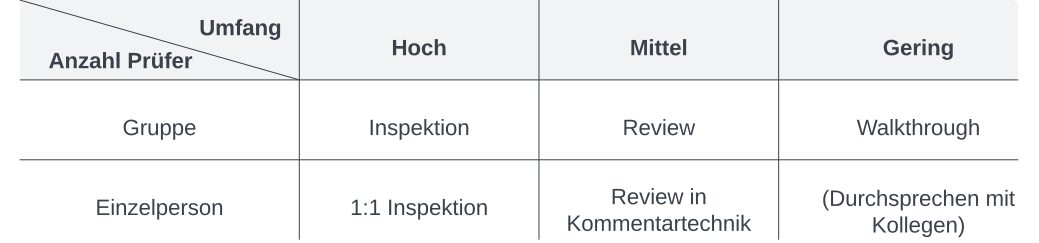
\includegraphics[scale=0.4]{part four/Manuelle Verfahren/img/manuelleverfahren}
    \caption{Verschiedene manuelle Verfahren, eingeordnet nach Anzahl der Teilnehmer und Umfang der Untersuchung. (Quelle: in Anlehnung an~\cite[Tab. 3.1, 17]{Wed09c})}
    \label{fig:manuelleverfahren}
\end{figure}

\noindent
\textbf{Inspektionen}, \textbf{Reviews} und \textbf{Walkthroughs} werden in Gruppen durchgeführt\footnote{
ergänzend führt \textit{Wedemann} als besonderes Verfahren \textbf{Pair Programming} an (vgl.~\cite[18]{Wed09c})
}.\\

\begin{itemize}
    \item \textbf{Inspektionen} sind \textbf{hoch formalisiert} und müssen von allen Beteiligten vorbereitet werden.
    \item Bei \textbf{Reviews} wird auf einen Teil der Formalisierung bei Vorbereitung und Durchführung verzichtet.\\
    \item In einem \textbf{Walkthrough} wird ein Artefakt von seinem Autor einer Gruppe von Mitarbeitern informell vorgestellt.
\end{itemize}

\section{Inspektion}
Die \textbf{Inspektion} ist das komplizierteste, aufwändigste, fromalisierteste und \textit{effektivste Verfahren}, um Defekte manuell aufzuspüren (vgl~\cite[18]{Wed09c}).\\
Alle anderen Verfahren basieren auf dem Verfahren der Inspektion.\\

\noindent
Aufgrund ihres Aufwandes kommen Inspektionen in der Praxis i.d.R. nur bei \textit{sehr wichtigen} Prüfgegenständen zum Einsatz.\\

\noindent
Bei der Inspektion wird von \textbf{Gutachtern} die \textbf{Erfüllung der Spezifikation} und die \textbf{Einhaltung von Standards} geprüft.\\
Damit nichts Wichtiges übersehen wird, werden Checklisten verwendet, die nicht unbedingt umfangreich sein müssen.\\
Die Inspektion findet zunächst alleine durch die jeweiligen Gutachter statt.
Die Ergebnisse werden in einer anschließenden \textbf{Inspektionssitzung} besprochen.

\begin{tcolorbox}[colback=white]
    Die Erarbeitung von Möglichkeiten zur Behebung von Defekten ist kein Teil der Inspektion.
\end{tcolorbox}

\subsection{Inspektionsteam}

\begin{itemize}
    \item \textbf{Moderator}: organisiert die Vorgänge der Inspektion, moderiert die Inspektionssitzung. Hat im besten Fall bereits Erfahungen mit Inspektionen gemacht und hat Kenntnisse in Gesprächsmoderation und strukturierter Arbeit mit Gruppen.
    \item \textbf{Autor(en)}: stehen während der Inspektion zur Beantwortung von Fragen zur Verfügung.
    \item \textbf{Inspektoren}: untersuchen den Prüfgegenstand, müssen also zu einer fachlichen Beurteilung in der Lage sein. Sind keine Vorgesetzten der Autoren.
    \item \textbf{Leser}: Einer der Inspektoren nimmt \textbf{während der Inspektionssitzung} die Rolle des \textbf{Lesers} ein, der durch den Prüfgegenstand führt.
\end{itemize}

\noindent
Wegen der Rollenverteilung \textbf{Leser}/\textbf{Inspektor} sollten mindestens zwei Inspektoren beteiligt sein.\\

\noindent
Das \textbf{Protokoll} führt der Moderator bei kleineren Inspektionsgruppen.\\
Bei größeren Gruppen (mehrere Inspektoren bzw. mehrere Autoren) übernimmt ein \textbf{dedizierter Protokollführer} diese Aufgabe.
\newpage


\newpage




	\glsaddall
	\printnoidxglossary[title=Glossar, toctitle=Glossar]

	\chapter{Manuelle Verfahren}


\section{Lernziele}

\begin{itemize}
    \item grundlegende Arten von qualitätssichernden Maßnahmen kennen
    \item grundlegende Arten von qualitätssichernden Maßnahmen nach verschiedenen Gesichtspunkten kategorisieren können
\end{itemize}

\newpage


\section{Einleitung}

Manuelle Verfahren sind ein effektives Mittel zur Suche nach Defekten.\\
Ihr Nachteil ist, dass ihre Durchführung sehr aufwändig ist.\\
Außerdem stellen manche Prüfarten für Menschen eher eintönige und fehleranfällige Tätigkeiten dar.\\

\noindent
Verschiedene Arten von Analysen können mit extra dafür entwickelten Werkzeugen automatisiert erfolgen, und lassen sich damit damit effizienter und zuverlässiger erledigen (vgl.~\cite[27]{Wed09c})

\noindent
Mit Hilfe der \textbf{werkzeuggestützten Analyse} kann u.a

\begin{itemize}
    \item die \textbf{Einhaltung von Programmierrichtlinien} überprüft werden
    \item nach \textbf{verdächtigen Mustern} im Code gesucht werden
    \item Defekte im Code aufspüren, die durch Fehlersituationen in Programmabläufen entstehen
\end{itemize}

\section{Überblick über die Verfahren}

Passende manuelle Verfahren gibt es für verschiedene Aufgabenstellungen und Teamgrößen: Besteht das Team nur aus wenigen Personen, reicht i.d.R. ein \textbf{Gutachter}.\\
Muss ein wichtiges Dokument geprüft werden (Anforderungsdokument als Vertragsgrundlage, zentraler, sicherheitskritischer Code), untersuchen mehrere Personen systematisch den Prüfgegenstand.\\

\noindent
Verschiedene Verfahren lassen sich nach der Anzahl der Teilnehmer und dem Umfang der Untersuchung einordnen (s. Abbildung~\ref{fig:manuelleverfahren} sowie Abschnitt~\ref{sec:andere-verfahren}).

\begin{figure}
    \centering
    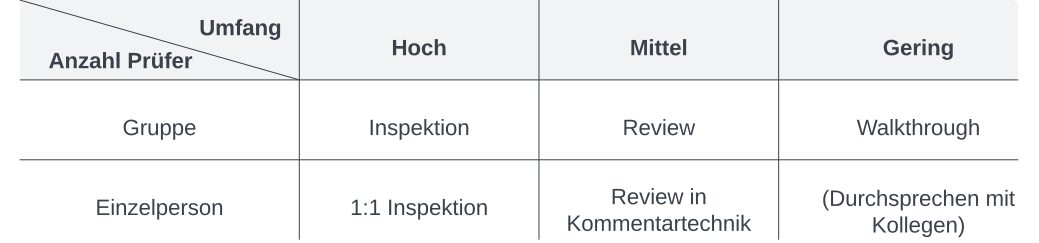
\includegraphics[scale=0.4]{part four/Manuelle Verfahren/img/manuelleverfahren}
    \caption{Verschiedene manuelle Verfahren, eingeordnet nach Anzahl der Teilnehmer und Umfang der Untersuchung. (Quelle: in Anlehnung an~\cite[Tab. 3.1, 17]{Wed09c})}
    \label{fig:manuelleverfahren}
\end{figure}

\noindent
\textbf{Inspektionen}, \textbf{Reviews} und \textbf{Walkthroughs} werden in Gruppen durchgeführt\footnote{
ergänzend führt \textit{Wedemann} als besonderes Verfahren \textbf{Pair Programming} an (vgl.~\cite[18]{Wed09c})
}.\\

\begin{itemize}
    \item \textbf{Inspektionen} sind \textbf{hoch formalisiert} und müssen von allen Beteiligten vorbereitet werden.
    \item Bei \textbf{Reviews} wird auf einen Teil der Formalisierung bei Vorbereitung und Durchführung verzichtet.\\
    \item In einem \textbf{Walkthrough} wird ein Artefakt von seinem Autor einer Gruppe von Mitarbeitern informell vorgestellt.
\end{itemize}

\section{Inspektion}
Die \textbf{Inspektion} ist das komplizierteste, aufwändigste, fromalisierteste und \textit{effektivste Verfahren}, um Defekte manuell aufzuspüren (vgl~\cite[18]{Wed09c}).\\
Alle anderen Verfahren basieren auf dem Verfahren der Inspektion.\\

\noindent
Aufgrund ihres Aufwandes kommen Inspektionen in der Praxis i.d.R. nur bei \textit{sehr wichtigen} Prüfgegenständen zum Einsatz.\\

\noindent
Bei der Inspektion wird von \textbf{Gutachtern} die \textbf{Erfüllung der Spezifikation} und die \textbf{Einhaltung von Standards} geprüft.\\
Damit nichts Wichtiges übersehen wird, werden Checklisten verwendet, die nicht unbedingt umfangreich sein müssen.\\
Die Inspektion findet zunächst alleine durch die jeweiligen Gutachter statt.
Die Ergebnisse werden in einer anschließenden \textbf{Inspektionssitzung} besprochen.

\begin{tcolorbox}[colback=white]
    Die Erarbeitung von Möglichkeiten zur Behebung von Defekten ist kein Teil der Inspektion.
\end{tcolorbox}

\subsection{Inspektionsteam}

\begin{itemize}
    \item \textbf{Moderator}: organisiert die Vorgänge der Inspektion, moderiert die Inspektionssitzung. Hat im besten Fall bereits Erfahungen mit Inspektionen gemacht und hat Kenntnisse in Gesprächsmoderation und strukturierter Arbeit mit Gruppen.
    \item \textbf{Autor(en)}: stehen während der Inspektion zur Beantwortung von Fragen zur Verfügung.
    \item \textbf{Inspektoren}: untersuchen den Prüfgegenstand, müssen also zu einer fachlichen Beurteilung in der Lage sein. Sind keine Vorgesetzten der Autoren.
    \item \textbf{Leser}: Einer der Inspektoren nimmt \textbf{während der Inspektionssitzung} die Rolle des \textbf{Lesers} ein, der durch den Prüfgegenstand führt.
\end{itemize}

\noindent
Wegen der Rollenverteilung \textbf{Leser}/\textbf{Inspektor} sollten mindestens zwei Inspektoren beteiligt sein.\\

\noindent
Das \textbf{Protokoll} führt der Moderator bei kleineren Inspektionsgruppen.\\
Bei größeren Gruppen (mehrere Inspektoren bzw. mehrere Autoren) übernimmt ein \textbf{dedizierter Protokollführer} diese Aufgabe.
\newpage


\newpage




%\input{chapters/ZusammenfassungAusblick}
% ...
%--------------------------------------------------------------------------
	\backmatter                        		% Anhang
%-------------------------------------------------------------------------

%\bibliographystyle{geralpha}			% Literaturverzeichnis
%\bibliography{literatur}     			% BibTeX-File literatur.bib
%\raggedright
	\sloppy
	\printbibliography
	\fussy

	\printindex


\end{document}
